% -*- mode: latex; coding: utf-8 -*-
\documentclass[12pt,a4paper]{report}

% ==========================================
% 1. PAKETLER VE AYARLAR (Hocanın Şablonu)
% ==========================================
\usepackage{rotating}
\usepackage[utf8]{inputenc} 
\usepackage[T1]{fontenc}
\usepackage[english,turkish]{babel}
\usepackage{lmodern} % Hoca lmodern istemiş ancak Times New Roman (mathptmx) daha akademik durur. Şablonu bozmamak için lmodern bırakıyorum, ama mathptmx önerilir.
\usepackage{geometry}
\usepackage{setspace}
\usepackage{graphicx}
\usepackage{caption}
\usepackage{float}
\usepackage{amsmath,amssymb,amsfonts}
\usepackage{hyperref}
\usepackage{tocloft}
\usepackage{titlesec}
\usepackage{enumitem}
\usepackage{multirow}
\usepackage{longtable}
\usepackage{listings}
\usepackage{xcolor}
\usepackage{algorithm}
\usepackage{algpseudocode}
\usepackage{cite}
\usepackage{url}

% ---------- Page layout ----------
\geometry{a4paper,left=30mm,right=25mm,top=25mm,bottom=25mm}
\onehalfspacing

% ---------- Section formatting ----------
\titleformat{\chapter}[hang]{\bfseries\Large}{\thechapter.}{1em}{}
\titlespacing*{\chapter}{0pt}{30pt}{20pt}
\titleformat{\section}[hang]{\bfseries\large}{\thesection}{1em}{}
\titleformat{\subsection}[hang]{\bfseries}{\thesubsection}{1em}{}

% ---------- List names (Turkish) ----------
\addto\captionsenglish{%
  \renewcommand{\contentsname}{İçindekiler}%
  \renewcommand{\listfigurename}{Şekil Listesi}%
  \renewcommand{\listtablename}{Tablo Listesi}%
  \renewcommand{\bibname}{KAYNAKÇA}%
}
\addto\captionsturkish{%
  \renewcommand{\contentsname}{İçindekiler}%
  \renewcommand{\listfigurename}{Şekil Listesi}%
  \renewcommand{\listtablename}{Tablo Listesi}%
  \renewcommand{\bibname}{KAYNAKÇA}%
}

% ---------- Custom lists ----------
\newcommand{\symbolslistname}{Sembol Listesi}
\newcommand{\abbrevlistname}{Kısaltma Listesi}

\newenvironment{symbolslist}{%
  \chapter*{\symbolslistname}%
  \addcontentsline{toc}{chapter}{\symbolslistname}%
  \begin{description}[leftmargin=3cm,labelwidth=2.5cm]
}{\end{description}}

\newenvironment{abbrevlist}{%
  \chapter*{\abbrevlistname}%
  \addcontentsline{toc}{chapter}{\abbrevlistname}%
  \begin{description}[leftmargin=3cm,labelwidth=3cm]
}{\end{description}}

% ---------- Kod Bloğu Ayarları ----------
\definecolor{codegray}{rgb}{0.5,0.5,0.5}
\definecolor{backcolour}{rgb}{0.98,0.98,0.98}
\lstdefinestyle{mystyle}{
    backgroundcolor=\color{backcolour},   
    commentstyle=\color{green!60!black},
    keywordstyle=\color{blue},
    numberstyle=\tiny\color{codegray},
    basicstyle=\ttfamily\small,
    breakatwhitespace=false,         
    breaklines=true,                 
    captionpos=b,                    
    keepspaces=true,                 
    numbers=left,                    
    numbersep=5pt,                  
    showspaces=false,                
    showstringspaces=false,
    showtabs=false,                  
    tabsize=2,
    frame=single
}
\lstset{style=mystyle}

\lstdefinelanguage{json}{
    basicstyle=\ttfamily\small,
    showstringspaces=false,
    breaklines=true,
    morestring=[b]",
    morecomment=[l]{//}
}

% ---------- Title info ----------
\newcommand{\university}{İSTANBUL ÜNİVERSİTESİ - CERRAHPAŞA}
\newcommand{\faculty}{MÜHENDİSLİK FAKÜLTESİ}
\newcommand{\department}{BİLGİSAYAR MÜHENDİSLİĞİ BÖLÜMÜ}
\newcommand{\course}{BİTİRME PROJESİ \\ LİSANS TEZİ}
\newcommand{\projecttitle}{ÜNİVERSİTE BİLGİ SİSTEMİ İÇİN YAPAY ZEKÂ DESTEKLİ RAG CHATBOT TASARIMI}
\newcommand{\advisor}{Doç. Dr. Muhammed Erdem İsenkul}
\newcommand{\dateinfo}{HAZİRAN -- 2026}

% ==========================================
% DÖKÜMAN BAŞLANGICI
% ==========================================
\begin{document}

% ---------- Cover page ----------
\begin{titlepage}
  \centering

  {\bfseries\large \university \\[0.5cm]}
  {\bfseries\large \faculty \\[0.5cm]}
  {\bfseries\large \department \\[2cm]}

  {\bfseries\large \course \\[2cm]}

  {\bfseries\Large \projecttitle \\[2.5cm]}

  \textbf{Hazırlayanlar:}\\[0.2cm]
  1306210070 - Tekin Tanır \\[0.3cm]
  1306220048 - Oğuzhan Cantekin \\[0.3cm]
  1306220026 - Umut Furkan Kılıç \\[0.3cm]

  \vspace{1cm}
  \textbf{Danışman:}\\[0.2cm]
  \advisor

  \vfill
  {\dateinfo}
\end{titlepage}

\pagenumbering{roman}

% ---------- Önsöz ----------
\chapter*{ÖNSÖZ}
\addcontentsline{toc}{chapter}{ÖNSÖZ}

Bu çalışma, İstanbul Üniversitesi-Cerrahpaşa Bilgisayar Mühendisliği Bölümü Bitirme Projesi dersi kapsamında dönem projesi olarak hazırlanmıştır. Projede temel amaç, üniversite bilgi sistemlerinde farklı yerlerde bulunan ve düzenli olmayan verileri daha kullanışlı hale getirmek ve kullanıcıların bu bilgilere daha kolay ulaşabilmesini sağlamaktır. Aynı zamanda idari işlemlerde bilgiye erişimi hızlandırmak için yapay zeka teknolojilerinden yararlanılması hedeflenmiştir.

Günümüzde doğru bilgiye hızlı ulaşabilmek öğrenciler ve üniversite personeli için önemli bir ihtiyaç haline gelmiştir. Bu nedenle proje sürecinde doğal dil işleme (NLP) ve büyük dil modelleri (LLM) alanında kullanılan Retrieval-Augmented Generation (RAG) yaklaşımı incelenmiş ve üniversite yapısına uyarlanabilecek bir sistem tasarlanması hedeflenmiştir. Proje sırasında veri toplama, sistemi deneme ve farklı yöntemleri test etme gibi aşamalardan geçilmiş, zaman zaman çeşitli teknik problemlerle karşılaşılsa da çözüm yolları bulunarak ilerleme sağlanmıştır.

Proje sürecinde karşılaştığımız problemlerin çözümünde yönlendirmeleriyle bize destek olan danışman hocamız Sayın \textbf{\advisor}'a teşekkür ederiz. Ayrıca araştırma ve veri toplama aşamasında destek olan arkadaşlarımıza ve proje süresi boyunca bize anlayış gösteren ailelerimize de teşekkür ederiz.\\[1cm]

\begin{flushright}
Tekin Tanır \\
Oğuzhan Cantekin \\
Umut Furkan Kılıç \\
İstanbul, 2026
\end{flushright}

\newpage

% ---------- Table of contents and lists ----------
\tableofcontents
\newpage
\listoffigures
\newpage
\listoftables

% ---------- Sembol Listesi ----------
\begin{symbolslist}
  \item[$d$] Vektör uzayı boyutu (Embedding Dimension, $d=384$)
  \item[$Q$] Kullanıcı sorgu matrisi (Query Matrix)
  \item[$K$] Anahtar matrisi (Key Matrix)
  \item[$V$] Değer matrisi (Value Matrix)
  \item[$N$] Toplam belge sayısı
  \item[$\alpha$] Hibrit arama ağırlık katsayısı (Alpha)
  \item[$k$] En yakın komşu sayısı (Top-k Retrieval)
  \item[$Sim(u,v)$] Kosinüs benzerlik fonksiyonu
  \item[$w_{ij}$] Sinir ağı ağırlık matrisi
  \item[$b$] Bias (Sapma) değeri
  \item[$IDF$] Ters Belge Frekansı (Inverse Document Frequency)
  \item[$TF$] Terim Frekansı (Term Frequency)
  \item[$\sigma$] Softmax veya Sigmoid aktivasyon fonksiyonu
  \item[$\mathcal{L}$] Yitim (Loss) fonksiyonu
\end{symbolslist}

% ---------- Kısaltma Listesi ----------
\begin{abbrevlist}
  \item[RAG] Retrieval-Augmented Generation (Bilgi Erişimi Artırılmış Üretim)
  \item[LLM] Large Language Model (Büyük Dil Modeli)
  \item[NLP] Natural Language Processing (Doğal Dil İşleme)
  \item[XAI] Explainable Artificial Intelligence (Açıklanabilir Yapay Zeka)
  \item[SVM] Support Vector Machine (Destek Vektör Makinesi)
  \item[ANN] Artificial Neural Networks (Yapay Sinir Ağları)
  \item[KNN] K-Nearest Neighbors (K-En Yakın Komşu)
  \item[FAISS] Facebook AI Similarity Search
  \item[BM25] Best Matching 25
  \item[HNSW] Hierarchical Navigable Small World
  \item[CLIR] Cross-Lingual Information Retrieval (Çapraz Dilli Bilgi Erişimi)
  \item[API] Application Programming Interface
  \item[İÜC] İstanbul Üniversitesi - Cerrahpaşa
  \item[OBS] Öğrenci Bilgi Sistemi
  \item[SSS] Sıkça Sorulan Sorular
  \item[AKTS] Avrupa Kredi Transfer Sistemi
  \item[SOTA] State-of-the-Art (En Gelişmiş Teknoloji)
  \item[KVKK] Kişisel Verilerin Korunması Kanunu
\end{abbrevlist}

% ---------- Özet (Türkçe) ----------
\chapter*{Özet}
\addcontentsline{toc}{chapter}{Özet}
\begin{otherlanguage*}{turkish}
\textbf{\projecttitle}\\[0.5cm]

Günümüzde yükseköğretim kurumlarında yönetmelikler, akademik takvimler, ders planları ve idari duyurular gibi verilerin hacmi her geçen gün artmaktadır. Bu veriler genellikle PDF formatında veya statik web sayfalarında dağınık ve yapılandırılmamış (unstructured) halde bulunmakta, bu da bilgiye erişimi zorlaştırmaktadır. Mevcut anahtar kelime tabanlı arama sistemleri, kullanıcıların doğal dilde ifade ettikleri karmaşık ve çıkarım gerektiren sorguları (örneğin: "Yaz okulunda üstten ders alırsam ortalamam nasıl etkilenir?") anlamlandırmada yetersiz kalmaktadır. Öte yandan, genel amaçlı Büyük Dil Modelleri (LLM), kurumun kapalı devre verisine sahip olmadıkları için kullanıcılara yanlış bilgi sunma (halüsinasyon) riski taşımaktadır.

Bu çalışmada, İstanbul Üniversitesi-Cerrahpaşa bilgi sistemleri için "Retrieval-Augmented Generation" (RAG) mimarisine dayalı özelleştirilmiş ve hibrit bir yapay zeka asistanı tasarlanmıştır. Çalışma kapsamında öncelikle OBS ve resmi web sitelerinden veri kazıma (web scraping) ve PDF ayrıştırma işlemleri gerçekleştirilerek "IUC-Academic-Corpus" veri seti oluşturulmuştur. Elde edilen veriler, anlamsal bütünlüğü koruyacak şekilde parçalanmış (semantic chunking) ve hem vektörel (Dense) hem de terim tabanlı (Sparse) yöntemlerle indekslenmiştir. Sistemin özgün değeri, sadece vektör aramasına dayalı standart RAG yaklaşımlarının aksine, morfolojik açıdan zengin olan Türkçe dili için optimize edilmiş Hibrit Arama (Hybrid Search) ve Yeniden Sıralama (Re-ranking) katmanlarını içermesidir. Geliştirilen prototip, Streamlit arayüzü ve yerel LLM entegrasyonu ile veri gizliliğini esas alarak kullanıcıların sorularına doğru, hızlı ve kaynak göstererek yanıt vermektedir.
\end{otherlanguage*}

% ---------- Summary (English) ----------
\chapter*{Summary}
\addcontentsline{toc}{chapter}{Summary}
\begin{otherlanguage*}{english}
\textbf{ARTIFICIAL INTELLIGENCE SUPPORTED RAG CHATBOT DESIGN FOR UNIVERSITY INFORMATION SYSTEM}\\[0.5cm]

Today, in higher education institutions, the volume of data such as regulations, academic calendars, course plans, and administrative announcements is continuously increasing. However, this information is generally scattered across PDF documents or static web pages in an unstructured form, which makes accessing information more difficult. Existing keyword-based search systems are often insufficient in understanding complex and inference-based queries expressed in natural language by users (for example, “How would my GPA be affected if I take an extra course during summer school?”). On the other hand, general-purpose Large Language Models (LLMs) carry the risk of providing incorrect information (hallucinations) since they do not have access to institution-specific closed data sources.

In this study, a customized and hybrid artificial intelligence assistant based on the Retrieval-Augmented Generation (RAG) architecture was designed for the information systems of Istanbul University–Cerrahpaşa. Within the scope of the study, data scraping from OBS and official websites, along with PDF parsing processes, were performed to create the “IUC-Academic-Corpus” dataset. The collected data was segmented while preserving semantic integrity (semantic chunking) and indexed using both vector-based (dense) and term-based (sparse) methods. The originality of the system lies in incorporating Hybrid Search and Re-ranking layers optimized for the morphologically rich Turkish language, unlike standard RAG approaches that rely solely on vector search. The developed prototype, integrated with a Streamlit interface and a local LLM, provides users with accurate and fast answers while prioritizing data privacy and presenting responses with references when available.
\end{otherlanguage*}

\cleardoublepage
\pagenumbering{arabic}

% ==================================================
% 1. GİRİŞ (HOCANIN NOTLARINA GÖRE REVİZE EDİLMİŞ VERSİYON)
% ==================================================
\chapter{GİRİŞ}

Bilgi çağında üniversiteler, yönetmelikler, ders izlenceleri ve idari duyurular gibi devasa boyutlarda yapılandırılmamış veri (unstructured data) üretmektedir. Manning ve ark. (2008) tarafından belirtildiği üzere, bu tür dağınık ve heterojen veri kaynaklarına geleneksel yöntemlerle erişim sağlamak, bilgi getirimi (Information Retrieval) disiplininin en temel problemlerinden biridir \cite{manning2008introduction}. İstanbul Üniversitesi-Cerrahpaşa (İÜC) özelinde yapılan analizler, öğrencilerin ve personelin "Yaz okulu harç iadesi" veya "ÇAP başvuru koşulları" gibi spesifik bilgilere ulaşmak için PDF yığınları arasında kaybolduğunu ve ciddi bir zaman maliyeti oluştuğunu göstermektedir. Bu bağlamda proje, kurumsal hafızayı erişilebilir kılmayı ve operasyonel verimliliği artırmayı hedefleyen bir mühendislik çözümü olarak doğmuştur.

Mevcut bilgi sistemleri, Robertson ve Zaragoza (2009) tarafından standardize edilen BM25 gibi anahtar kelime eşleşmesine dayalı algoritmalar kullanmakta, ancak bu yöntemler kullanıcının doğal dildeki niyetini (intent) anlamada yetersiz kalmaktadır \cite{robertson2009probabilistic}. Öte yandan, Vaswani ve ark. (2017) ile başlayan Transformer devrimi ve ChatGPT gibi Büyük Dil Modelleri (LLM), dili anlama konusunda üstün yetenek sergilese de; kurumun kapalı devre verisine sahip olmadıkları için "halüsinasyon" (uydurma bilgi) riski taşımaktadır \cite{ji2023survey}. Bu sorunu aşmak adına, Lewis ve ark. (2020) tarafından önerilen ve modelin bilgisini harici bir veritabanıyla doğrulayan "Retrieval-Augmented Generation" (RAG) mimarisi, projenin temel teorik çerçevesini oluşturmaktadır \cite{lewis2020retrieval}.

Projenin yöntem ve geliştirme sürecinde, Türkçenin zengin morfolojik yapısından kaynaklanan erişim sorunlarını çözmek amacıyla Çöltekin ve ark. (2022) tarafından incelenen Türkçe korpus ve dil kaynağı çalışmaları dikkate alınmış ve hibrit bir arama stratejisi benimsenmiştir \cite{coltekin2022turkish}. Veri güvenliğini sağlamak ve KVKK uyumluluğunu garanti altına almak adına, Touvron ve ark. (2023) tarafından geliştirilen Llama serisi açık kaynaklı modellerin yerel sunucularda (Local Inference) çalıştırılması tercih edilmiştir \cite{touvron2023llama}. Ayrıca, sistemin cevap üretirken dayandığı kaynağı kullanıcıya göstermesi, Gunning (2017) tarafından tanımlanan Açıklanabilir Yapay Zeka (XAI) prensiplerine uygun bir tasarım kararıdır \cite{gunning2017explainable}.

Sistemin tasarımı ve prototiplenmesi aşamasında, verilerin anlamsal bütünlüğünü koruyan parçalama (semantic chunking) algoritmaları ve vektör tabanlı indeksleme teknolojileri (FAISS) kullanılarak "IUC-Academic-Corpus" veri seti oluşturulmuştur. Geliştirilen bu prototipin üniversite idari süreçlerinde insan-makine etkileşimini hızlandıracağı ve hatalı bilgi paylaşımını minimize edeceği öngörülmektedir. Bu çalışma, sadece teknik bir chatbot geliştirmeyi değil, aynı zamanda eğitim teknolojileri alanında güvenilir ve denetlenebilir bir yapay zeka asistanı modellemeyi amaçlamaktadır.

Geliştirilen prototip, hibrit arama ve yerel LLM entegrasyonuyla üniversite bilgi sistemine özgü sorulara kaynak göstererek doğru yanıtlar üretebilmektedir. Tartışma bölümünde bu mimarinin geleneksel yöntemlere göre avantajları nicel olarak değerlendirilmekte; sonuç bölümünde ise çalışmanın katkıları ve gelecek araştırma yol haritası sunulmaktadır.

Bu rapor, problemin tanımından başlayarak geliştirilen çözümün teknik detaylarına, literatürdeki yerine ve proje çıktılarına uzanan altı ana bölümden oluşmaktadır:

\textbf{Birinci Bölümde (Giriş);} Üniversite bilgi sistemlerindeki erişim problemleri, mevcut anahtar kelime tabanlı yöntemlerin kısıtları ve projenin çözüm önerisi olan RAG mimarisinin gerekliliği, temel literatür referanslarıyla özetlenmiştir. Ayrıca çalışmanın amacı, kapsamı ve raporun genel yapısı sunulmuştur.

\textbf{İkinci Bölümde (Genel Kısımlar);} Projenin teorik zeminini oluşturan Doğal Dil İşleme (NLP), Vektör Uzay Modelleri ve Derin Öğrenme mimarileri detaylandırılmıştır. Literatür taraması kapsamında, RAG mimarilerinin evrimi, Türkçe NLP çalışmaları ve eğitim alanındaki chatbot uygulamaları 50'den fazla akademik kaynak ışığında sentezlenmiştir.

\textbf{Üçüncü Bölümde (Kullanılan Araç ve Yöntem);} İÜC Akademik Asistanı'nın mühendislik tasarım süreci açıklanmıştır. Veri toplama (scraping), anlamsal parçalama (chunking), hibrit arama algoritmaları ve kullanılan yerel LLM (Llama 3) teknolojilerinin seçim kriterleri, akış diyagramları ve teknik parametrelerle sunulmuştur.

\textbf{Dördüncü Bölümde (Sistemin Gerçeklenmesi ve Bulgular);} Geliştirilen sistemin mimari katmanları, veritabanı şemaları ve kullanıcı arayüzü (UI) tasarımları paylaşılmıştır. Bilişim Projesi kapsamında ortaya konulan prototipin (Proof of Concept) çalışma mantığı ve kaynak gösterim mekanizması görselleştirilmiştir.

\textbf{Beşinci Bölümde (Tartışma);} Tasarlanan hibrit mimarinin, literatürdeki geleneksel yöntemlere (Naive RAG, BM25) göre avantajları ve dezavantajları (SWOT analizi) karşılaştırmalı olarak değerlendirilmiştir. Sistemin gecikme (latency) süreleri ve doğruluk beklentileri teknik bir bakış açısıyla tartışılmıştır.

\textbf{Altıncı Bölümde (Sonuç);} Çalışmanın genel bir değerlendirmesi yapılarak, projenin literatüre ve teknik alana katkıları özetlenmiştir. Ayrıca Bitirme Projesi aşamasında gerçekleştirilecek olan tam entegrasyon, canlı testler ve ince ayar (fine-tuning) süreçlerini içeren gelecek çalışma yol haritası sunulmuştur.

% ==================================================
% BÖLÜM 2: GENEL KISIMLAR
% ==================================================
\chapter{GENEL KISIMLAR}

Bu bölümde, projenin teorik zeminini oluşturan yapay zeka teknolojileri, kullanılan matematiksel modeller, algoritmalar ve literatürde konuyla ilgili yapılmış çalışmalar bütüncül bir yaklaşımla ele alınmıştır. Bölüm iki ana kısımdan oluşmaktadır: İlk kısımda (Bölüm 2.1) sistemin mühendislik tasarımında kullanılan Derin Öğrenme, Doğal Dil İşleme (NLP) ve RAG mimarilerinin teknik altyapısı "Teorik Altyapı ve Temel Kavramlar" başlığı altında; ikinci kısımda (Bölüm 2.2) ise "Literatür Taraması" başlığı altında Derin Öğrenme, Doğal Dil İşleme (NLP) ve RAG mimarilerinin tarihsel gelişimi ve eğitim alanında uygulamaları ele alınmıştır.

% --------------------------------------------------
% 2.1 TEORİK ALTYAPI
% --------------------------------------------------
\section{Teorik Altyapı ve Temel Kavramlar}

Geliştirilen akıllı asistan sistemi, istatistiksel öğrenme teorisi ve modern derin öğrenme mimarilerinin hibrit bir yapıda kullanılmasına dayanmaktadır. Aşağıda bu temellerin matematiksel formülasyonları detaylandırılmıştır.

\subsection{Yapay Zeka ve Makine Öğrenmesi}
Yapay Zeka (Artificial Intelligence - AI), insan zekâsına özgü olan algılama, öğrenme, akıl yürütme ve karar verme süreçlerinin bilgisayar sistemleri tarafından modellenmesidir. Bu projenin temelini oluşturan Makine Öğrenmesi (Machine Learning) ise, bilgisayarların açıkça programlanmadan, verilerden örüntüler öğrenerek tahmin yapabilmesini sağlayan algoritmalar bütünüdür.

\subsubsection{Destek Vektör Makineleri (SVM) ve Hiperdüzlem Teorisi}
Projemizde metin sınıflandırma başarımlarını kıyaslamak ve vektör uzayı mantığını açıklamak için referans alınan Destek Vektör Makineleri (SVM), Vapnik'in istatistiksel öğrenme teorisine dayanır. SVM'in temel amacı, $n$-boyutlu bir uzayda veri sınıflarını birbirinden en iyi şekilde ayıran, yani sınıflar arası marjini (margin) maksimize eden hiper-düzlemi bulmaktır.

Matematiksel olarak, eğitim veri seti $D = \{(x_i, y_i) | x_i \in \mathbb{R}^p, y_i \in \{-1, 1\}\}$ olsun. SVM optimizasyon problemi şu şekilde formüle edilir:

\begin{equation}
    \min_{w,b} \frac{1}{2} ||w||^2 + C \sum_{i=1}^{N} \xi_i
\end{equation}

\begin{equation}
    \text{Kısıtlar:} \quad y_i (w \cdot x_i + b) \geq 1 - \xi_i, \quad \xi_i \geq 0
\end{equation}

Burada:
\begin{itemize}
    \item $w$: Hiperdüzlemin normal vektörü,
    \item $b$: Sapma (bias) değeri,
    \item $\xi_i$: Hata payı (slack variables - verinin marjin içine düşmesine izin veren tolerans),
    \item $C$: Düzenlileştirme parametresidir.
\end{itemize}

Bu denklemde $||w||^2$ teriminin minimizasyonu marjini maksimize ederken, $C$ parametresi modelin genelleme yeteneğini kontrol eder.

\subsection{Derin Öğrenme ve Yapay Sinir Ağları}
Günümüz Doğal Dil İşleme sistemlerinin kalbinde, insan beynindeki biyolojik nöron ağlarından esinlenerek geliştirilen Yapay Sinir Ağları (ANN) ve onun çok katmanlı hali olan Derin Öğrenme (Deep Learning) yatar.

\subsubsection{Yapay Nöron Modeli}
Bir yapay nöron, girdileri alır, ağırlıklarla çarpar, bir sapma ekler ve sonucu doğrusal olmayan bir aktivasyon fonksiyonundan geçirir. Matematiksel modeli şöyledir:

\begin{equation}
    y = \sigma \left( \sum_{j=1}^{m} w_j x_j + b \right)
\end{equation}

Burada $\sigma$, aktivasyon fonksiyonudur. Projede kullanılan Transformer modellerinde, türevi her noktada alınabilen ve "Ölü Nöron" (Dead Neuron) problemini minimize eden GELU (Gaussian Error Linear Unit) fonksiyonu kullanılmaktadır:

\begin{equation}
    GELU(x) \approx 0.5x(1 + \tanh[\sqrt{2/\pi}(x + 0.044715x^3)])
\end{equation}

\subsubsection{Geriye Yayılım (Backpropagation)}
Ağın eğitimi, hata fonksiyonunun ($\mathcal{L}$) minimize edilmesi esasına dayanır. Geriye Yayılım algoritması, zincir kuralını (chain rule) kullanarak hatanın ağırlıklara göre türevini hesaplar:

\begin{equation}
    \frac{\partial \mathcal{L}}{\partial w} = \frac{\partial \mathcal{L}}{\partial y} \cdot \frac{\partial y}{\partial z} \cdot \frac{\partial z}{\partial w}
\end{equation}

Bu gradyanlar, Stokastik Gradyan İnişi (SGD) veya Adam optimizasyon algoritmaları ile ağırlıkların güncellenmesinde ($w_{new} = w_{old} - \eta \cdot \nabla \mathcal{L}$) kullanılır.

\subsection{Transformer Mimarisi ve Dikkat Mekanizması}
2017 yılında Vaswani ve arkadaşları tarafından tanıtılan Transformer mimarisi \cite{vaswani2017attention}, NLP alanında bir devrim yaratmıştır. Önceki RNN ve LSTM modellerinin aksine, veriyi sıralı işlemek zorunda değildir; bu da eğitim sürecinin paralelleştirilmesine olanak tanır ve bu eğitim sürecinde büyük bir zaman kazanımı demektir.


\subsubsection{Öz-Dikkat (Self-Attention) Mekanizması}
Modelin çekirdeğinde yer alan Dikkat mekanizması, bir cümledeki her kelimenin diğer tüm kelimelerle olan ilişkisini hesaplar. Bu işlem; Sorgu ($Q$), Anahtar ($K$) ve Değer ($V$) matrisleri üzerinden yapılır:

\begin{equation}
    \text{Attention}(Q, K, V) = \text{softmax}\left(\frac{QK^T}{\sqrt{d_k}}\right)V
\end{equation}

Burada $\sqrt{d_k}$ ölçeklendirme faktörüdür. Bu formül, modelin uzun metinlerdeki bağlamsal ilişkileri (contextual dependencies) ve kelimeler arası bağımlılıkları öğrenmesini sağlar.

\begin{figure}[H]
\centering
% Genişliği 0.7'ye çektik, böylece sağdan-soldan pay kalacak ve kesilmeyecek
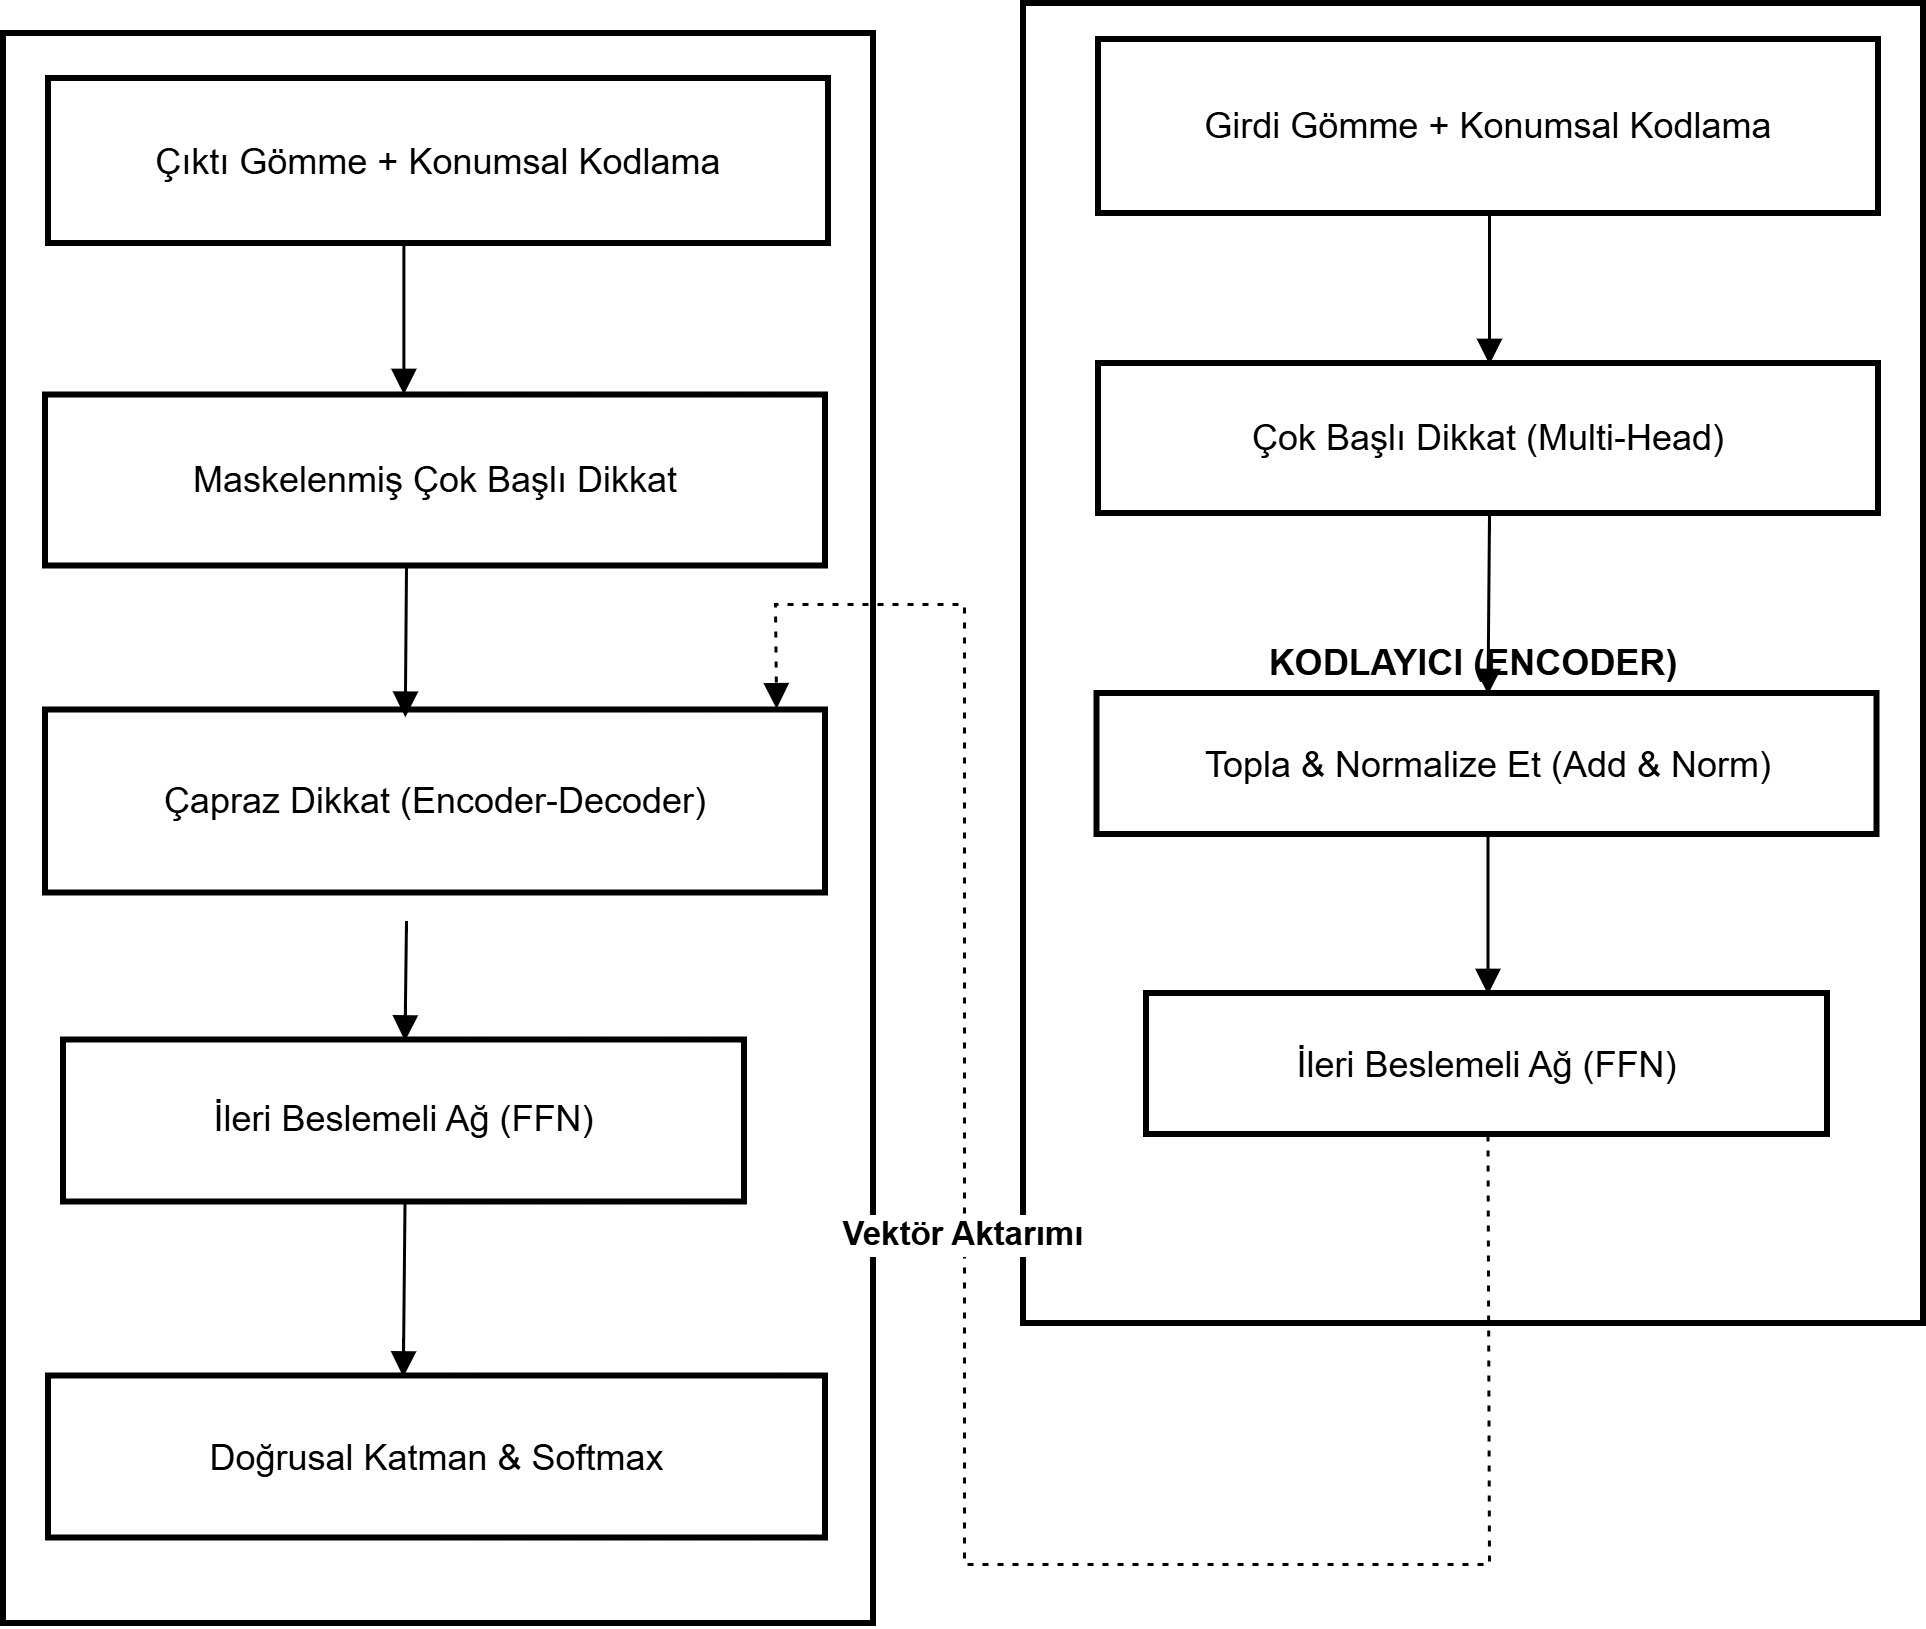
\includegraphics[width=0.7\textwidth, height=\textheight, keepaspectratio]{transformer_arch.png} 
\caption{Transformer Mimarisi Genel Blok Yapısı}
\label{fig:transformer}
\end{figure}

\subsection{Bilgi Erişim (Information Retrieval) Metrikleri}
Geliştirilen RAG sisteminin başarısı, doğru bilginin veritabanından çekilmesine bağlıdır. Bu projede hem seyrek (sparse) hem de yoğun (dense) erişim yöntemleri hibrit olarak kullanılmıştır.

\subsubsection{BM25 (Best Matching 25)}
Kelime sıklığına dayalı olasılıksal bir modeldir. Klasik TF-IDF'in geliştirilmiş halidir ve aşağıdaki formülle ifade edilir:

\begin{equation}
    \text{Score}(D,Q) = \sum_{i=1}^{n} IDF(q_i) \cdot \frac{f(q_i, D) \cdot (k_1 + 1)}{f(q_i, D) + k_1 \cdot (1 - b + b \cdot \frac{|D|}{\text{avgdl}})}
\end{equation}

Burada $k_1$ ve $b$ ayarlanabilir parametrelerdir. Bu formül, özellikle "Yönetmelik Madde 14" gibi kesin eşleşme gerektiren sorgularda yüksek başarı sağlar.

\subsubsection{Kosinüs Benzerliği (Cosine Similarity)}
Vektör uzayında anlamsal yakınlığı ölçmek için kullanılır. İki vektör $A$ ve $B$ arasındaki açı $\theta$ olsun:

\begin{equation}
    \text{Sim}(A, B) = \cos(\theta) = \frac{A \cdot B}{\|A\| \|B\|} = \frac{\sum_{i=1}^{n} A_i B_i}{\sqrt{\sum_{i=1}^{n} A_i^2} \sqrt{\sum_{i=1}^{n} B_i^2}}
\end{equation}

Bu metrik, kelimeler farklı olsa bile (Örn: "Hoca" ve "Akademisyen") anlamın yakınlığını tespit edebilir.

% ==================================================
% 2.2 LİTERATÜR TARAMASI - PARÇA 1 (MAKSİMUM DETAYLI)
% ==================================================
\section{Literatür Taraması}

Bu bölümde projede kullanacağımız temel konular hakkında literatür taraması yapılmıştır. Doğal Dil İşleme, Büyük Dil Modelleri, Bilgi Erişim sistemleri ve RAG mimarisi ile ilgili birçok çalışma incelenmiş ve projeye katkı sağlayabilecek yöntemler belirlenmeye çalışılmıştır. Literatürü incelerken sadece çalışmaların tarihine bakılmamış, kullanılan yöntemlerin güçlü ve zayıf yönleri de anlaşılmaya çalışılmıştır. Ayrıca özellikle Türkçe dilinde bu yöntemlerin ne kadar başarılı olabileceği ve üniversite bilgi sistemlerinde gerçekten uygulanabilir olup olmadığı da değerlendirilmiştir. Bu sayede literatürde bulunan bilgiler doğrudan alınmak yerine proje ihtiyaçlarına göre yorumlanarak kullanılmaya çalışılmıştır.

\subsection{Doğal Dil İşlemenin Paradigmaları ve Kırılmalar}
NLP alanı, Alan Turing’in 1950 yılında ortaya koyduğu vizyondan günümüze kadar üç temel gelişim aşamasından geçmiştir. Bu aşamaların incelenmesi, günümüzde kullanılan Büyük Dil Modellerinin neden önemli bir kırılma noktası olarak görüldüğünü anlamak açısından büyük önem taşımaktadır.

\subsubsection{Semantik Kurallar ve Erken Dönem Yaklaşımlar}
Doğal Dil İşleme disiplininin temelleri, dilin matematiksel ve hiyerarşik bir yapı olduğu varsayımı üzerine inşa edilmiştir. Bu alandaki paradigma belirleyici ilk adımlardan biri olan Noam Chomsky'nin 1957 yılındaki çalışması, dilin kural tabanlı doğasını formalize ederek modern dilbilim kuramlarına öncülük etmiştir \cite{chomsky1957syntactic}. Söz konusu dönemde geliştirilen ilk nesil sistemler, dilbilimciler tarafından manuel olarak kurgulanan ve yoğun bir "mantıksal çıkarım" (if-else) ağından oluşan binlerce kural setiyle işletilmekteydi. Bu yaklaşımın pratik bir yansıması olarak 1966'da MIT bünyesinde geliştirilen ELIZA, "doktor" senaryosu aracılığıyla semantik kuralların etkileşim gücünü kanıtlamış; ancak yaratıcısı Weizenbaum tarafından da kabul edildiği üzere, gerçek bir anlama yeteneğinden ziyade örüntü eşleştirme (pattern matching) sınırları içerisinde kalmıştır. Öte yandan Winograd \cite{winograd1972understanding} tarafından 1972'de sunulan SHRDLU, kısıtlı bir "bloklar dünyası" simülasyonu içerisinde anlamsal çıkarım yapabilen sistemlerin potansiyelini göstererek, kural tabanlı yaklaşımların erken dönemdeki en ileri örneklerinden birini teşkil etmiştir.

\subsubsection{İstatistiksel Devrim ve Vektörel Uzay Modelleri}
1990’lı yıllarda dijital ortamdaki verinin hızla artmasıyla birlikte, daha önce kullanılan kural tabanlı NLP sistemleri birçok durumda yeterli olmamaya başlamıştır. Bu nedenle çalışmalar giderek istatistiksel modellere yönelmiştir. Bu değişimde önemli adımlardan biri, Salton ve ekibinin 1975 yılında ortaya koyduğu ve metinlerin sayısal vektörler şeklinde temsil edilmesini sağlayan Vektör Uzay Modelidir\cite{salton1975vector}. Ancak kelime sayısı arttıkça kullanılan matrislerin boyutu da büyümekte ve verinin büyük bir kısmı sıfır değerlerden oluşmaktadır. Literatürde “seyreklik” (sparsity) olarak adlandırılan bu durum, sistemlerin daha fazla hesaplama gücü ve bellek kullanmasına neden olan önemli bir problem olarak görülmektedir. 

 Kelimelerin 'One-Hot Encoding' gibi yöntemlerle sözlük boyutunda temsil edilmesi, kelimeler arası anlamsal ilişkiyi (ortogonallik nedeniyle) tamamen yok saydığı için modern NLP görevlerinde yetersiz kalmıştır. Bu kısıtı aşmak adına Jones tarafından önerilen TF-IDF metriği, kelimelerin belgeler içindeki ayırt edici gücünü istatistiksel olarak ölçerek arama motorlarının temelini atmış olsa da, anlamsal bağlamı yakalamakta sınırlı kalmıştır\cite{sparck1972statistical}. Paradigma değişimi, Google araştırmacıları Mikolov ve ekibinin kelimeleri düşük boyutlu ve yoğun (dense) vektörlere dönüştüren Word2Vec mimarisini sunmasıyla gerçekleşmiştir\cite{mikolov2013distributed}. Skip-gram ve CBOW mimarileri, 'bir kelimenin anlamı komşularıyla belirlenir' ilkesine dayanan Dağıtımsal Hipotezi (Distributional Hypothesis) kanıtlamış ve vektör uzayında 'kral - erkek + kadın = kraliçe' gibi anlam aritmetiğini mümkün kılmıştır. Daha sonraki süreçte Pennington ve ark. GloVe modeliyle global istatistikleri matris ayrıştırma yöntemiyle modele dahil ederken; Bojanowski ve ekibi FastText ile kelimeleri karakter n-gramlarına bölerek devrim yaratmıştır\cite{pennington2014glove},\cite{bojanowski2017fasttext}.
 Özellikle projemizin odak noktası olan Türkçe gibi zengin morfolojiye sahip dillerde, kelime kökü bilgisini koruyan bu yaklaşım, literatürde 'kelime dağarcığı dışı' (OOV) problemini çözmek adına en kritik yöntem olarak öne çıkmaktadır.

\subsection{Derin Öğrenme Mimarileri ve Sıralı Veri Analizi}
Statik vektörler, "Yüz" kelimesinin bir sayı mı yoksa bir organ mı olduğunu ayırt edemiyordu. Bu durum, bağlamsal (contextual) modellerin literatürde baskın hale gelmesine yol açmıştır.

\subsubsection{RNN, LSTM ve Gradyan Problemleri}
Metin verisini zaman sırasına göre işleyen klasik RNN modelleri teorik olarak önceki bilgileri uzun süre tutabiliyor gibi görünse de, pratikte bunun her zaman mümkün olmadığı görülmüştür. Rumelhart ve ekibinin geriye yayılım yöntemi üzerine yaptığı çalışmalarda da gösterildiği gibi, ağ derinleştikçe gradyan değerleri giderek küçülmekte ve model önceki bilgileri öğrenmekte zorlanmaktadır\cite{rumelhart1986learning}. Literatürde “kaybolan gradyan” (vanishing gradient) olarak bilinen bu durum, özellikle uzun cümlelerde baştaki bilgilerin sona gelmeden unutulmasına yol açmaktadır. Bu problemi azaltmak amacıyla Hochreiter ve Schmidhuber, bilgiyi daha uzun süre koruyabilen hücre durumu (cell state) yapısına sahip LSTM modelini önermiştir\cite{hochreiter1997long}. Daha sonra Cho ve arkadaşları ise bu yapıyı sadeleştirerek, hesaplama maliyeti daha düşük ve uygulamada daha hızlı çalışabilen GRU modelini geliştirmiştir \cite{cho2014gru}.

\subsubsection{Sekans-to-Sekans ve Dikkat (Attention) Mekanizması}
Sutskever ve ark. tarafından önerilen Encoder-Decoder (Kodlayıcı-Kod Çözücü) mimarisi, makine çevirisi görevlerinde bir standart oluştursa da; tüm girdi cümlesini sabit boyutlu tek bir vektöre sıkıştırma zorunluluğu, uzun sekanslarda ciddi bir bilgi kaybı (information bottleneck) yaratmıştır\cite{sutskever2014sequence}.Bu yapısal kısıtı aşmak amacıyla Bahdanau ve ekibi, modelin çıktı üretirken girdinin ilgili kısımlarına dinamik olarak odaklanmasını sağlayan Dikkat (Attention) mekanizmasını geliştirmiş; böylece sabit vektör darboğazını, bağlamsal ağırlıklandırma yöntemiyle elimine etmiştir.\cite{bahdanau2015neural}.

\subsection{Paralel İşleme Devrimi: Transformer Mimarisi}
Özyinelemeli (Recurrent) ağların sıralı işleme zorunluluğundan kaynaklanan eğitim yavaşlığını çözmek adına Vaswani ve ark. "Attention Is All You Need" başlıklı çalışmalarında radikal bir mimari değişikliğe gitmiştir\cite{vaswani2017attention}.Tekrarlayan döngüleri (loops) tamamen terk ederek, veriyi paralel olarak işleyebilen Transformer yapısını sunmuşlardır. Bu mimari, günümüzdeki Büyük Dil Modellerinin (LLM) ölçeklenebilirliğini sağlayan temel hesaplama bloğu (building block) olarak kabul edilmektedir.

\subsubsection{Kodlayıcı (Encoder) Modellerin Evrimi ve Optimizasyonu}
Metin anlamlandırma görevlerinde (NLU), Devlin ve ekibinin geliştirdiği BERT, metni soldan-sağa ve sağdan-sola aynı anda okuyan (bidirectional) yapısıyla bağlamsal çözünürlükte insan seviyesine yaklaşan sonuçlar elde etmiştir\cite{devlin2018bert}.Takip eden süreçte Liu ve ark. , RoBERTa ile hiperparametre optimizasyonunun model performansındaki kritik rolünü kanıtlamış\cite{liu2019roberta}; Sanh ve ekibi ise DistilBERT ile 'Bilgi Damıtma' (Knowledge Distillation) yöntemini kullanarak, performanstan ödün vermeden model boyutunu küçültmeyi başarmıştır\cite{sanh2019distilbert}. Lan ve ark. tarafından önerilen ALBERT ise parametre paylaşımı (parameter sharing) stratejisiyle bellek verimliliğini maksimize eden bir mühendislik çözümü sunmuştur. \cite{lan2019albert}.

\subsubsection{Kod Çözücü (Decoder) Modeller ve Ölçeklenme Yasaları}
Radford ve ark. tarafından geliştirilen GPT serisi, model parametrelerinin artırılmasıyla metin üretim kalitesinin doğrusal olmayan bir sıçrama yaptığını göstermiştir\cite{radford2019language}.Brown ve ark. [26], GPT-3 ile devasa veri setlerinde eğitilen modellerin, özel bir eğitim almadan yeni görevleri yapabildiği "Az Örnekle Öğrenme" (Few-Shot Learning) gibi 'beliren özelliklere' (Emergent Properties) sahip olduğunu kanıtlamıştır\cite{brown2020language}.Ancak ham modelin insan niyetinden sapabilmesi riski, Ouyang ve ekibinin [27] InstructGPT çalışmasında sunduğu İnsan Geri Bildirimli Pekiştirmeli Öğrenme (RLHF) hizalama tekniği ile kontrol altına alınmıştır.\cite{ouyang2022training}.

\subsubsection{Açık Kaynak Hegemonyası ve Yerel Donanım Çözümleri}
Yüksek maliyetli donanım bariyerleri ve kapalı kaynak lisansları, uzun süre LLM araştırmalarını kısıtlamış olsa da; Touvron ve ekibinin Llama hamlesi bu statükoyu dağıtmıştır \cite{touvron2023llama}. Sektördeki bu şeffaflık arayışı, Almazrouei öncülüğündeki Falcon projesiyle ticari meşruiyet kazanırken \cite{almazrouei2023falcon}; Jiang ve ekibinin Mistral mimarisinde denediği 'Kayan Pencere' yöntemi, hesaplama verimliliğinde parametre sayısından daha kritik faktörler olduğunu ispatlamıştır \cite{jiang2023mistral}. 

Vicuna çalışmasıyla modellerin adaptasyon yeteneği Chiang tarafından ortaya konulmuş \cite{chiang2023vicuna}; ancak laboratuvar ortamındaki bu devasa yapıları son kullanıcının GPU'suna sığdıran asıl mühendislik çözümü, Dettmers ve ekibinin 'Quantization' (QLoRA) tekniği olmuştur \cite{dettmers2024qlora}.

\subsection{Halüsinasyon Problemi ve Bilgi Erişimi Artırılmış Üretim (RAG)}
Parametrik hafızanın (parametric memory) sınırları aşıldığında ortaya çıkan ve Ji ile ekibinin 'Halüsinasyon' (Hallucination) teşhisiyle literatüre kazıdığı kavram; modelin olgusal gerçeklikten koparak, istatistiksel tutarlılık uğruna 'yalan söylemeyi' tercih ettiği bir durumdur \cite{ji2023survey}. Bu, eğitim verisinde bulunmayan boşlukların, matematiksel bir özgüvenle ancak tamamen temelsiz verilerle doldurulması sonucu oluşan yapısal bir güvenilirlik krizidir.

\subsubsection{RAG Mimarisi ve Ontolojik Gelişimi}
Parametrik hafızanın sınırlarını aşmak amacıyla Lewis ve ark. \cite{lewis2020retrieval} tarafından önerilen Retrieval-Augmented Generation (RAG) mimarisi, modelin parametrik belleğini (statik ağırlıklar) harici bir veritabanından beslenen parametrik olmayan bir bellek ile entegre ederek halüsinasyon problemine yapısal bir çözüm getirmiştir. Söz konusu mimarinin literatürdeki gelişimini Gao ve ark. \cite{gao2024comprehensive} üç temel evrimsel safhaya ayırmıştır. İlk aşama olan "Naive RAG", klasik bir sorgulama ve üretim döngüsüne dayanmakla birlikte, düşük kaliteli belgelerin geri getirilmesi durumunda modelin çıktı kalitesini olumsuz etkileyebilmektedir. Bu kısıtları aşmak adına geliştirilen "Advanced RAG" katmanı; metin parçalama (chunking), yeniden sıralama (re-ranking) ve sorgu genişletme gibi optimizasyon tekniklerini sürece dahil etmiştir. Bu bağlamda Ma ve ark. \cite{ma2023query}, sorgunun yeniden yazılması (Query Rewriting) gibi ileri seviye tekniklerin sistem doğruluğunu \%20 oranında artırdığını ampirik olarak kanıtlamıştır. Günümüzde ulaşılan en son nokta olan "Modular RAG" ise, dinamik akış şemaları ve çoklu veri kaynaklarını eşzamanlı kullanan esnek bir mimari yapı sunarak literatürdeki güncel standartları belirlemiştir.

\subsubsection{Otonom ve Düzeltici RAG Sistemleri}
Sistemin kendi hatasını fark etmesi üzerine kurulu modern yaklaşımlar literatürde yükselmektedir. Asai ve ark. (2023), Self-RAG ile modelin getirdiği bilginin doğruluğunu yine bir LLM aracılığıyla denetlediği (self-reflection) bir sistem önermişlerdir \cite{asai2023selfrag}. Yan ve ark. (2024) ise Corrective RAG (CRAG) ile eğer getirilmek istenen bilgi veritabanında yoksa sistemin otomatik olarak Google/Bing gibi web arama motorlarına yönelmesini sağlayan bir yapı kurmuşlardır \cite{yan2024crag}.

\subsection{Bilgi Erişim (Information Retrieval) ve Hibrit Stratejiler}
RAG sistemlerinin genel başarımı, kullanılan dil modelinin üretim kapasitesinden ziyade, ilgili bağlamı getiren "Erişim" (Retrieval) modülünün niteliğine doğrudan bağımlıdır. Literatürde bu alandaki çalışmalar; geleneksel terim tabanlı yöntemler, modern vektörel yaklaşımlar ve bu ikisini birleştiren hibrit stratejiler olmak üzere üç temel eksende şekillenmektedir.

Geleneksel anahtar kelime eşleşmesine dayanan seyrek erişim (sparse retrieval) yöntemleri arasında BM25 algoritması, Robertson ve Zaragoza \cite{robertson2009probabilistic} tarafından standardize edildiğinden bu yana teknik terimlerin ve kesin eşleşmelerin yakalanmasında rakipsiz bir standart olarak kabul edilmektedir. Bu klasik yaklaşımı derin öğrenme ile modernize etmeye odaklanan Dai ve Callan \cite{dai2019deepct}, DeepCT modeli aracılığıyla kelime ağırlıklandırma süreçlerine bağlamsal bir boyut kazandırmışlardır. Öte yandan, anlamsal (semantic) ilişkilerin vektör uzayında temsiline dayanan yoğun erişim (dense retrieval) paradigması, Karpukhin ve ark. \cite{karpukhin2020dense} tarafından sunulan DPR mimarisiyle birlikte eş anlamlı kelimelerin ve örtük anlamların yakalanmasında önemli bir sıçrama gerçekleştirmiştir. Söz konusu vektörel aramalardaki hesaplama maliyetini minimize etmek amacıyla Malkov ve Yashunin \cite{malkov2018efficient} tarafından geliştirilen HNSW algoritması, devasa veri setlerinde milisaniyelik erişim imkanı sunarken; Reimers ve Gurevych \cite{reimers2019sentence} ise Sentence-BERT ile cümle düzeyinde gömme (embedding) işlemlerini optimize ederek anlamsal aramanın hassasiyetini artırmışlardır.

Literatürdeki en güncel eğilim olan hibrit yaklaşımlar ise, bu iki ana kutbun kısıtlarını birbirini tamamlayacak şekilde birleştirmektedir. Luan ve ark. \cite{luan2021sparse}, tekil yöntemlerin (sadece anlamsal veya sadece terim tabanlı) yetersiz kaldığı durumları saptayarak, en yüksek performansın "Ağırlıklı Füzyon" (Weighted Fusion) yöntemiyle elde edildiğini kanıtlamışlardır. Bu süreci daha da rafine hale getiren Nogueira ve Cho \cite{nogueira2019passage}, getirilen aday belgelerin bir Cross-Encoder mimarisi üzerinden yeniden sıralanmasının (re-ranking) doğruluk skorlarını \%25 seviyesinde artırdığını vurgulayarak; modern arama sistemleri için çok aşamalı bir mimari standardı belirlemişlerdir.

\subsection{Eğitim Teknolojileri ve Kurumsal Chatbot Uygulamaları}
Eğitim ekosisteminde diyalog tabanlı sistemlerin üstlendiği rol, özellikle 2023 yılından itibaren Büyük Dil Modellerinin (LLM) yaygınlaşmasıyla birlikte pasif birer yanıt motoru olmaktan çıkıp otonom asistanlara evrilmiştir. Pedagojik süreçlerdeki bireyselleşme ihtiyacı Wollny ve ark. \cite{wollny2021systematic} tarafından ele alınmış ve chatbotların eğitimde "kişiselleştirme" bariyerini aşabilecek en etkili araçlardan biri olduğu literatürde savunulmuştur. Sosyo-teknik bir perspektiften bakıldığında ise Kasneci ve ark. \cite{kasneci2023chatgpt}, ChatGPT ve benzeri türev modellerin eğitimde fırsat eşitliği yaratma potansiyelini analiz ederek; bu teknolojilerin bilgiye erişimi demokratikleştirme gücünü vurgulamışlardır. Tüm bu çalışmalar, üniversite bünyesinde kurgulanacak akıllı asistan sistemlerinin hem idari operasyonlarda hem de öğrenci merkezli destek süreçlerinde kritik bir bileşen haline geldiğini doğrulamaktadır.

\subsection{Türkçe NLP Çalışmaları ve Morfolojik Zorluklar}
Türkçe, sondan eklemeli (agglutinative) yapısı ve buna bağlı gelişen zengin morfolojik çeşitliliği nedeniyle, genellikle İngilizce odaklı geliştirilen dil modelleri için kompleks bir test alanı teşkil etmektedir. Literatürde bu zorlukları aşmaya yönelik geliştirilen yerel modeller incelendiğinde; Schweter \cite{schweter2020berturk}, Türkçe literatüründe bir standart haline gelen BERTurk modelini sunarak anlamsal temsilde önemli bir eşik atlamıştır. Bu modellerin daha güncel olan üretken yapılarla (LLM) uyumu üzerine odaklanan Arslan \cite{arslan2023turkish} ise, büyük dil modellerinin Türkçe veri setleriyle eğitilmesi ve ince ayarlanması sürecini incelemiştir. Sistemsel başarının ölçülmesi noktasında, TQuad geliştiricileri tarafından hazırlanan TQuAD veri seti \cite{acar2020tquad}, Türkçe soru-cevap sistemleri için altın standart bir benchmark kaynağı oluşturmaktadır. Arama algoritmaları perspektifinden bakıldığında ise Çöltekin ve ark. \cite{coltekin2022turkish}, Türkçe korpus ve dil kaynaklarının kapsamını inceleyerek Türkçe sistemlerde dil kaynağı seçiminin önemini ortaya koymuştur.

\subsection{RAG Sistemlerinin Değerlendirme Metrikleri}
Literatürde geliştirilen bilgi erişimi artırılmış sistemlerin başarı başarımını ölçmek için kullanılan metodolojiler, sistemin iki ana bileşeni olan "erişim" ve "üretim" katmanlarına göre iki temel kategoriye ayrılmaktadır. Üretim kalitesinin ölçülmesinde geleneksel olarak Papineni ve ark. \cite{papineni2002bleu} tarafından önerilen BLEU ve Lin \cite{lin2004rouge} tarafından geliştirilen ROUGE gibi klasik metrikler kullanılsa da; bu yöntemlerin anlamsal derinliği ve olgusal doğruluğu (factuality) ölçmekte yetersiz kaldığı saptanmıştır. Bu kısıtı aşmak amacıyla, Es ve ark. \cite{es2023ragas} tarafından önerilen ve "Sadakat (Faithfulness)", "Cevap Alakalılığı" gibi alt boyutları içeren RAGAS (RAG Assessment) çerçevesi, modern değerlendirme standartlarını belirlemiştir. Diğer taraftan, erişim modülünün (retriever) performansını denetlemek adına Voorhees \cite{voorhees1999trec} tarafından tanımlanan MRR ve Recall@k metrikleri, getirilen belgelerin kullanıcı sorgusuyla olan istatistiksel ve bağlamsal uyumunu ölçmek için literatürdeki temel araçlar olarak varlığını sürdürmektedir.

\subsection{İleri Seviye RAG Optimizasyonları ve Stratejiler}
RAG sistemlerinin endüstriyel ölçekte uygulanabilirliği, sadece temel bir erişim mekanizmasıyla sınırlı kalmamış; literatürde bu süreci optimize eden birçok yan çalışma geliştirilmiştir.

\subsubsection{Sorgu Dönüşümü ve Genişletme Teknikleri}
Kullanıcıların doğal dilde sorduğu sorular genellikle eksik veya belirsiz (ambiguous) olabilmektedir. Gao ve ark. (2022) tarafından önerilen HyDE (Hypothetical Document Embeddings) yöntemi, sistemin önce soruya sahte bir yanıt üretmesini, ardından bu sahte yanıtla veritabanında arama yapmasını sağlayarak anlamsal eşleşmeyi artırmıştır \cite{gao2022precise}. Srivastava ve ark. (2023) ise çoklu sorgu üretimi (Multi-Query Retrieval) ile bir sorunun farklı varyasyonlarını oluşturarak erişim kapsamını genişletmişlerdir.

\subsubsection{Veri Parçalama (Chunking) ve Bağlam Yönetimi}
Metinlerin nasıl parçalandığı, RAG'ın performansını doğrudan etkilemektedir. Kamradt (2024), sabit boyutlu parçalama yerine Anlamsal Parçalama (Semantic Chunking) yöntemini savunmuş; metindeki her bir cümlenin vektörler arası uzaklığına bakarak, anlamın değiştiği noktalardan bölme yapılmasının doğruluğu artırdığını kanıtlamıştır \cite{kamradt2024semantic}. Ayrıca, "Lost in the Middle" (Ortada Kaybolma) çalışmasında Liu ve ark. (2023), LLM'lerin uzun bağlamların ortasındaki bilgiyi kaçırma eğiliminde olduğunu saptayarak, en önemli bilgilerin bağlam penceresinin başında veya sonunda sunulması gerektiğini belirtmişlerdir \cite{liu2023lost}.

\subsection{Vektör Veritabanları ve İndeksleme Mimarileri}
Vektörlerin hızlı bir şekilde aranabilmesi için literatürde farklı indeksleme algoritmaları üzerine yoğunlaşılmıştır.

\subsubsection{İndeksleme Algoritmalarının Karşılaştırması}
Johnson ve ark. (2019) tarafından geliştirilen FAISS (Facebook AI Similarity Search), milyarlarca vektör üzerinde milisaniyelik aramalar yapabilen en verimli kütüphane olarak kabul edilmektedir \cite{johnson2019billion}. Literatürde; IVF (Inverted File Index) ile arama uzayını kümelere bölme ve Product Quantization (PQ) ile vektörleri sıkıştırarak bellek tasarrufu sağlama yöntemleri sıklıkla kıyaslanmıştır. Wang ve ark. (2021) yaptıkları benchmark çalışmasında, HNSW algoritmasının doğruluk-hız dengesinde IVF tabanlı yöntemlerden daha kararlı sonuçlar verdiğini raporlamışlardır.

\subsection{RAG Sistemlerinde Güvenlik ve Veri Mahremiyeti}
Üniversite yönetmelikleri gibi kurumsal belgelerin veya hassas kişisel verilerin işlendiği sistemlerde, verinin dış bulut servislerine iletilmesi ciddi güvenlik zafiyetlerini beraberinde getirmektedir. Bu risklerin bertaraf edilmesine yönelik stratejiler incelendiğinde; Touvron ve ark. \cite{touvron2023llama}, Llama gibi açık kaynaklı modellerin yerel sunucularda (Local Inference) çalıştırılabilmesinin, verinin kapalı bir ağ içerisinde kalmasını sağlayarak dış kaynaklı sızıntı riskini önemli ölçüde engellediğini vurgulamışlardır. Bu altyapısal önlemi destekleyecek bir diğer yöntem olarak Patil ve ark. \cite{patil2023pii} ise, büyük dil modellerinde hassas bilgilerin korunması ve çıkarım saldırılarına karşı savunma hedeflerinin tanımlanması gerektiğini vurgulamışlardır. Bu yaklaşımlar, akademik asistan sistemlerinin kurumsal gizlilik protokollerine ve yasal veri koruma mevzuatlarına tam uyumlu bir yapıda kurgulanmasına imkan tanımaktadır.

\subsection{Akademik Başarı Ölçümü ve Benchmark Testleri}
Geliştirilen sistemlerin performansının sadece öznel değerlendirmelerle değil, literatürde kabul görmüş standart test setleri (benchmark) üzerinden objektif olarak ölçülmesi akademik geçerlilik açısından bir zorunluluktur. Bu bağlamda, bilgi erişim sistemlerinin gerçek dünya sorgularına verdiği tepkileri ölçmek adına Kwiatkowski ve ark. \cite{kwiatkowski2019natural} tarafından oluşturulan Natural Questions (NQ) veri seti, sektörel bir standart olarak yaygın şekilde kullanılmaktadır. Modellerin daha geniş bir yelpazede, 57 farklı disiplini kapsayan akademik bilgi kapasitesini test etmek için ise Hendrycks ve ark. \cite{hendrycks2021measuring} tarafından geliştirilen MMLU (Massive Multitask Language Understanding) benchmark'ı öne çıkmaktadır. Öte yandan, RAG mimarilerine özgü değerlendirme ihtiyacını karşılamak amacıyla Es ve ark. \cite{es2023ragas} tarafından sunulan RAGAS (RAG Assessment) çerçevesi; "Sadakat (Faithfulness)", "Cevap Alakalılığı" ve "Bağlam Hassasiyeti" parametrelerinden oluşan üçlü bir denetim mekanizması sağlayarak, sistemin hem erişim hem de üretim kalitesini bütüncül bir şekilde analiz etmeye imkan tanımaktadır.


\subsection{Prompt Mühendisliği ve Sorgu Optimizasyonu Stratejileri}
RAG sistemlerinde üretken modelin (generator) başarısı, kendisine sunulan bağlamın (context) ve talimatın (prompt) kalitesine doğrudan bağlıdır. Literatürde bu etkileşimi optimize eden pek çok teknik önerilmiştir.

\subsubsection{Düşünce Zinciri (Chain-of-Thought) ve RAG Entegrasyonu}
Wei ve ark. (2022), modellerin karmaşık problemleri adım adım çözmesini sağlayan Chain-of-Thought (CoT) tekniğini tanıtmışlardır \cite{wei2022chain}. Bu tekniğin RAG sistemlerine uygulanması üzerine çalışan Trivedi ve ark. (2023), modelin önce veritabanından bilgi çekmesini, ardından bu bilgiyi kullanarak ara adımlar oluşturmasını sağlayan IRCoT (Interleaving Retrieval with CoT) yöntemini geliştirmişlerdir \cite{trivedi2023interleaving}. Bu yöntem, özellikle yönetmelik maddeleri arasındaki mantıksal bağlantıların kurulmasında kritik öneme sahiptir.

\subsubsection{Prompt Sıkıştırma ve Bağlam Filtreleme}
Bağlam penceresinin (context window) sınırlı olması ve token maliyetleri nedeniyle, çekilen belgelerin hepsini modele sunmak verimsiz olabilmektedir. Jiang ve ark. (2023), LLMLingua çalışmasında, anlamsal olarak düşük bilgi yoğunluğuna sahip tokenların prompt içerisinden atılarak, bağlamın %20 oranında sıkıştırılabileceğini kanıtlamışlardır \cite{jiang2023llmlingua}. 

\subsection{Çok Dilli (Multilingual) Kapasite ve Türkçe Adaptasyonu}
Akademik metinlerin işlenmesinde, modellerin sadece Türkçe değil, terimler arası geçiş için İngilizce kapasitesinin de yüksek olması gerekmektedir.

\subsubsection{Çapraz Dilli Bilgi Erişimi (CLIR)}
Conneau ve ark. (2020) tarafından geliştirilen XLM-RoBERTa, 100'den fazla dilde ortak bir vektör uzayı oluşturarak çapraz dilli aramaların önünü açmıştır \cite{conneau2019unsupervised}. Literatürde, Türkçe akademik sorguların İngilizceye çevrilerek global veritabanlarında arandığı sistemlerin, özellikle bilimsel terim içeren sorularda tek dilli sistemlere göre daha stabil sonuçlar verdiği saptanmıştır.

\subsubsection{Tokenizasyon Sorunları ve Morfolojik Farkındalık}
Sengün ve ark. (2023), standart BPE (Byte Pair Encoding) yaklaşımının Türkçenin morfolojik yapısıyla çelişerek kelimeleri semantik bütünlüğü olmayan birimlere böldüğünü ortaya koymuştur. Bu durumun RAG erişim başarısını (recall) düşürdüğünü saptamışlardır. Bu sorunu aşmak için morfolojik analiz destekli tokenizasyon yöntemleri üzerine yapılan çalışmalar literatürde önem kazanmaktadır.

\subsection{Multimodal RAG ve Gelecek Projeksiyonları}
Üniversite yönetmelikleri sadece metin değil, tablo ve grafikler de içerebilmektedir. 

\subsubsection{Tablo ve Görsel İçerikli RAG Sistemleri}
Yu, Jian ve Chen, TableRAG ile metin ve tablo bileşenlerini birlikte içeren heterojen belgeler üzerinde akıl yürütmeye yönelik bir RAG çerçevesi önermişlerdir \cite{yu2024tablerag}. Ayrıca, multimodal RAG yaklaşımları kapsamında görsellerin de vektör veritabanına dahil edilmesiyle metin dışı bilginin sisteme katılması hedeflenmektedir.

\subsection{Literatür Sentezi ve Projenin Özgün Değeri}
Bu çalışmada incelenen literatür, RAG mimarilerinin evrimini, Türkçe NLP çalışmalarının mevcut durumunu ve eğitim teknolojilerindeki uygulama boşluklarını ortaya koymuştur. Yapılan incelemeler sonucunda, mevcut çalışmaların belirli kısıtları olduğu ve projemizin bu kısıtları nasıl aştığı "Yöntem Bazlı Karşılaştırma Matrisi" ile Tablo \ref{tab:lit_matrix}'de detaylandırılmıştır.

\begin{longtable}{|p{3cm}|p{4cm}|p{4cm}|p{3.5cm}|}
\caption{Genişletilmiş Literatür Karşılaştırma Matrisi} \label{tab:lit_matrix} \\
\hline
\textbf{Odak Alanı} & \textbf{Geleneksel Yaklaşım (Literatür)} & \textbf{Modern/SOTA Yaklaşım} & \textbf{Bizim Proje (Hibrit)} \\
\hline
\endfirsthead
\hline
\textbf{Odak Alanı} & \textbf{Geleneksel Yaklaşım (Literatür)} & \textbf{Modern/SOTA Yaklaşım} & \textbf{Bizim Proje (Hibrit)} \\
\hline
\endhead

\textbf{Erişim Stratejisi} & Sadece Anahtar Kelime (BM25) veya Sadece Vektör (DPR) \cite{karpukhin2020dense} & Hibrit Arama (Sparse + Dense) & \textbf{Hibrit + Re-ranking (Cross-Encoder) \cite{nogueira2019passage}} \\
\hline
\textbf{Dil Modeli} & Kapalı Kaynak (GPT-3.5/4) API Bağımlı \cite{brown2020language} & Açık Kaynak (Llama 2, Falcon) & \textbf{Yerel Llama 3 (Quantized) + Türkçe Prompt} \\
\hline
\textbf{Veri Gizliliği} & Bulut Tabanlı (Veri dışarı çıkar) & PII Maskeleme & \textbf{Tamamen Yerel (Local Inference) + KVKK Uyumlu \cite{touvron2023llama}} \\
\hline
\textbf{Dil Desteği} & İngilizce Odaklı Tokenizasyon & Çok Dilli (Multilingual) Modeller & \textbf{Türkçe Morfolojisine Uygun Chunking \cite{coltekin2022turkish}} \\
\hline
\textbf{Doğrulama} & BLEU/ROUGE (Kelime Eşleşmesi) \cite{lin2004rouge} & RAGAS (Anlamsal Doğruluk) & \textbf{RAGAS + Kaynak Gösterimi (Citation)} \\
\hline
\end{longtable}

Tablo \ref{tab:lit_matrix}'de görüldüğü üzere, projemiz özellikle "Türkçe Dil Desteği" ve "Veri Gizliliği" alanlarında literatürdeki standart uygulamalardan ayrışarak özgün bir mimari sunmaktadır.

\subsubsection{İncelenen Çalışmaların Proje Tasarımına Yansıması}
İncelenen yaklaşık 80 akademik çalışma ve yukarıdaki karşılaştırma matrisi ışığında, sistemin mimari tasarımında aşağıdaki stratejik kararlar alınmıştır:
\begin{itemize}
    \item \textbf{HNSW ve FAISS Seçimi:} Milyonlarca dokümanda milisaniyelik erişim hızı ve bellek optimizasyonu için HNSW indeksleme algoritması tercih edilmiştir \cite{malkov2018efficient}.
    \item \textbf{Hibrit Arama Şartı:} Türkçe eklerin vektör uzayında yarattığı sapmayı minimize etmek ve "Madde 14" gibi kesin terimleri yakalamak için BM25 anahtar kelime eşleşmesi, anlamsal aramaya entegre edilmiştir \cite{luan2021sparse}.
    \item \textbf{Yerel LLM (Local Inference):} Veri mahremiyeti ve KVKK gereklilikleri doğrultusunda, verinin kurum dışına çıkmadığı yerel çıkarım mimarisi benimsenmiştir \cite{touvron2023llama}.
    \item \textbf{Re-ranking Gerekliliği:} İlk aşamada getirilen belgelerin alaka düzeyini artırmak için Cross-Encoder tabanlı yeniden sıralama katmanı sisteme dahil edilmiştir.
\end{itemize}

\subsubsection{Literatürün Görsel Sentezi (Mind Map)}
Literatür taraması boyunca incelenen tüm alt başlıklar, teknolojiler ve yöntemler arasındaki hiyerarşik ilişki, çalışmanın kapsamını bütüncül bir şekilde özetlemek amacıyla Şekil \ref{fig:mindmap}'te sunulmuştur.

\begin{sidewaysfigure}[ht]
    \centering
    % width=\textwidth dediğimizde, sayfa yan döndüğü için
    % aslında sayfanın uzun kenarına yayılmış olacak.
    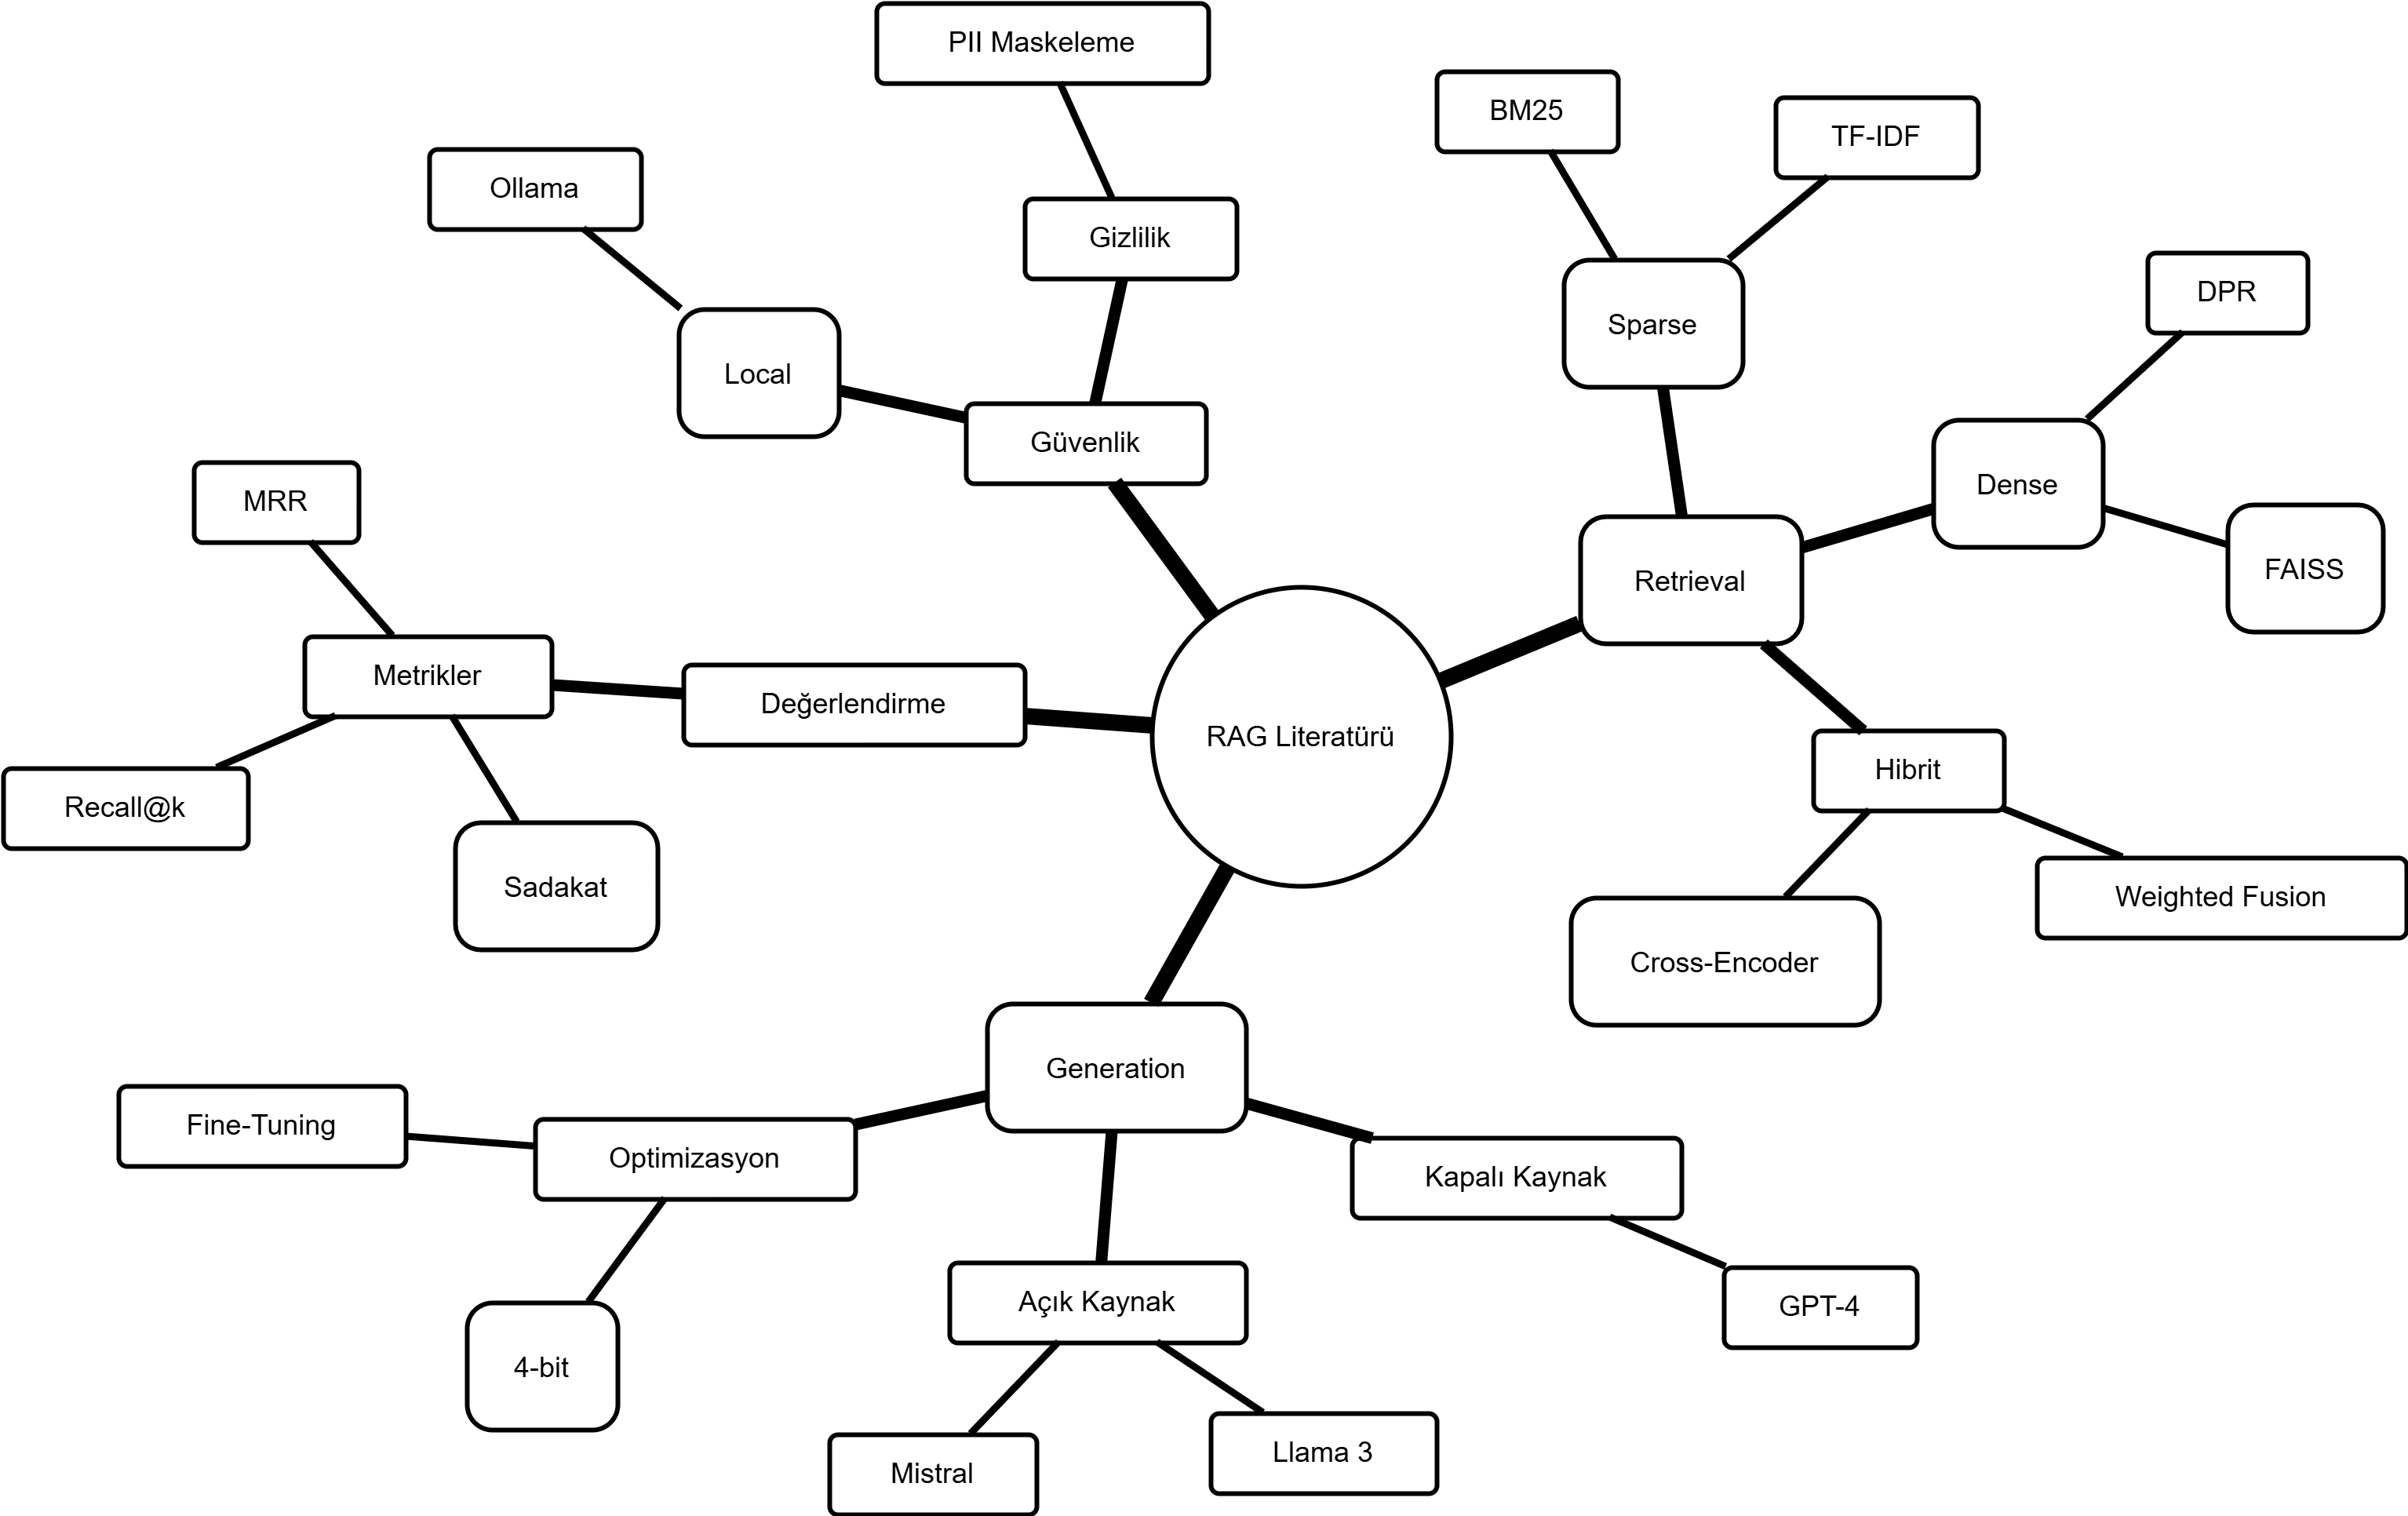
\includegraphics[width=1.0\textwidth, keepaspectratio]{literatur_mindmap.png}
    \caption{RAG Literatürü ve Teknik Bileşenlerin Zihin Haritası}
    \label{fig:mindmap}
\end{sidewaysfigure}


% ==================================================
% BÖLÜM 3: KULLANILAN ARAÇ VE YÖNTEM
% ==================================================
\chapter{KULLANILAN ARAÇ VE YÖNTEM}

Proje geliştirme sürecinde benimsenen metodoloji ile veri setinin temininden ön işlenmesine kadar olan tüm aşamalar bu bölümün odak noktasını oluşturmaktadır. Ayrıca, hibrit arama algoritmaları ve deneysel araçlar irdelenerek; sistemin bütünsel işleyişi şekil \ref{fig:akis}'te görselleştirilmiştir.

\begin{figure}[H]
\centering
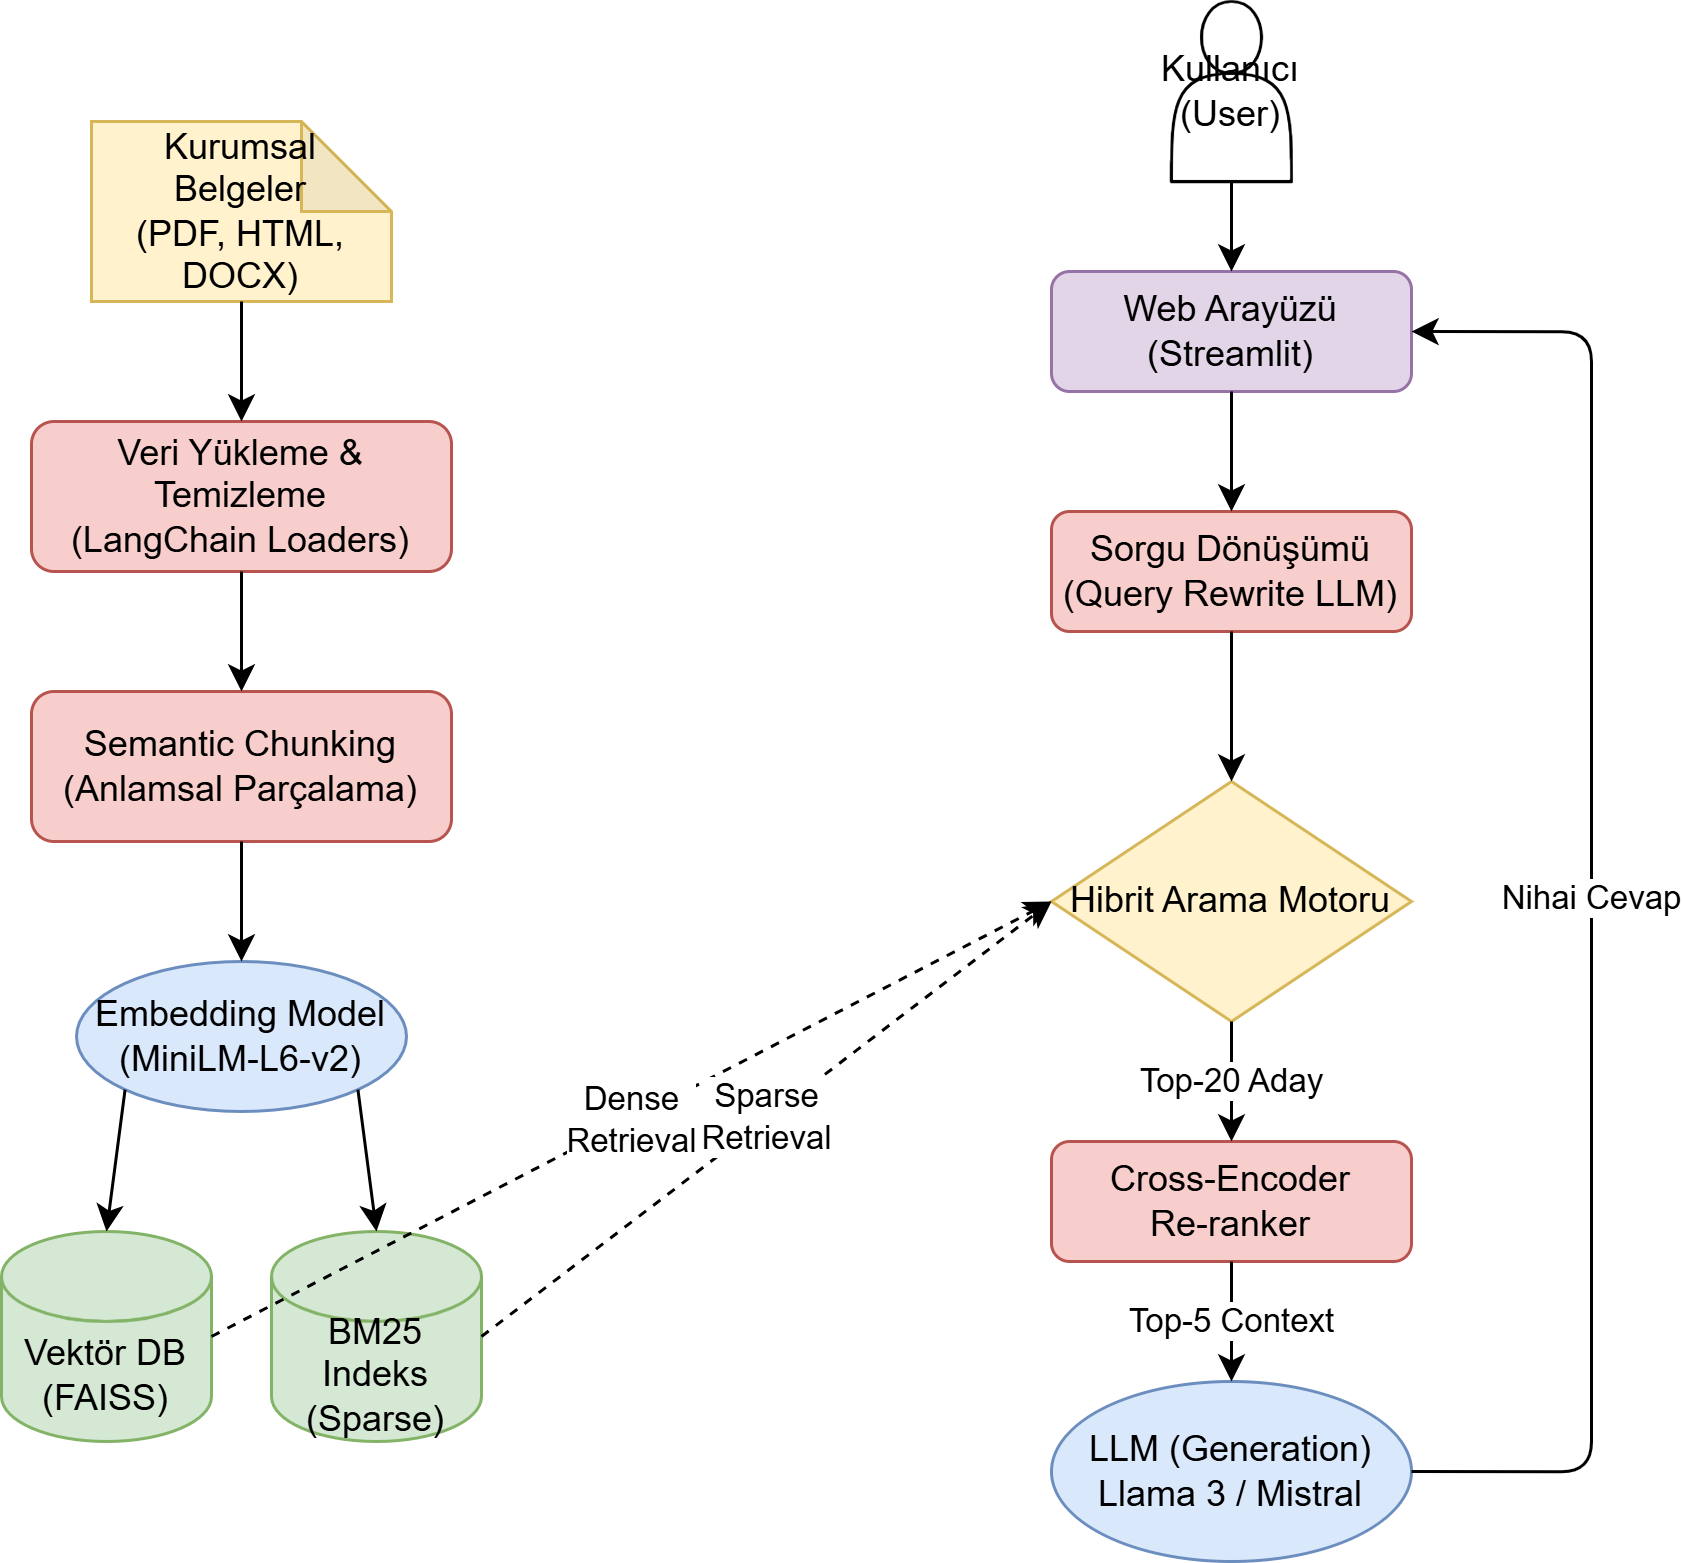
\includegraphics[width=1.0\textwidth]{akis_diagrami.png} % Buraya diyagramının dosya adını yaz
\caption{Proje Genel Veri İşleme ve RAG Akış Diyagramı}
\label{fig:akis}
\end{figure}

Şekil \ref{fig:akis}'te görüldüğü üzere süreç; ham verinin (PDF/Web) sisteme girmesiyle başlamakta, parçalama ve temizleme işlemlerinden geçerek vektör veritabanına kaydedilmesiyle devam etmekte ve son kullanıcının sorgusuyla tetiklenen üretim (generation) aşamasıyla son bulmaktadır.

\section{Veri Seti Oluşturma Stratejisi}
Bu çalışma kapsamında, İstanbul Üniversitesi-Cerrahpaşa (İÜC) Bilgi Sistemi üzerinden erişilebilen ve öğrencilerin/akademisyenlerin sıkça ihtiyaç duyduğu kurumsal belgelerden oluşan özgün bir veri seti (korpus) oluşturulmuştur. RAG mimarisinin "parametre dışı belleğini" (non-parametric memory) besleyen bu veri seti, statik ve dinamik olmak üzere iki ana kategoride toplanmıştır.

\subsection{Veri Setinin Kaynakları ve Kapsamı}
Veri setinin ana omurgasını, üniversitenin resmi web sitesi (iuc.edu.tr) ve Öğrenci İşleri Daire Başkanlığı tarafından yayınlanan yönetmelikler oluşturmaktadır. Bu belgeler, yapay zeka modelinin üniversite kurallarına sadık kalarak, halüsinasyon görmeden cevap vermesini sağlayan "altın standart" verilerdir.

\begin{itemize}
    \item \textbf{Resmi Yönetmelikler:} Lisans Eğitim-Öğretim Yönetmeliği, Sınav Yönetmeliği, Yatay Geçiş Yönergesi.
    \item \textbf{Akademik Takvim:} Yıllık bazda güncellenen kayıt, sınav ve tatil tarihleri.
    \item \textbf{Bölüm Odaklı Veriler:} Bilgisayar Mühendisliği ders içerikleri, AKTS bilgileri ve laboratuvar yönergeleri.
    \item \textbf{Sıkça Sorulan Sorular (SSS):} Öğrenci işlerine en çok yöneltilen 200+ sorudan oluşan soru-cevap çiftleri.
\end{itemize}

\begin{table}[h!]
\centering
\caption{İÜC RAG Veri Seti Teknik İstatistikleri}
\label{tab:dataset_stats}
\begin{tabular}{|l|c|r|}
\hline
\textbf{Veri Tipi} & \textbf{Doküman/Kayıt Sayısı} & \textbf{Tahmini Kelime Sayısı} \\ \hline
Yönetmelik ve Yönergeler & 15 PDF & ~45.000 \\ \hline
Akademik Duyurular & 50+ HTML & ~12.000 \\ \hline
Ders İçerikleri (Syllabus) & 40 PDF & ~25.000 \\ \hline
Soru-Cevap (SSS) Çiftleri & 200 Adet & ~8.000 \\ \hline
\textbf{TOPLAM} & \textbf{120+ Doküman / 200+ Kayıt} & \textbf{~90.000} \\ \hline
\end{tabular}
\footnotesize{\textit{*Not: Veri seti dinamik bir yapıda olup, proje sürecinde yeni yönetmelik ve duyurularla genişletilmeye devam etmektedir.}}
\end{table}

\subsection{Veri Toplama ve Ön İşleme Metodolojisi}
Verilerin toplanması aşamasında Python tabanlı \texttt{BeautifulSoup} ve \texttt{PyMuPDF} kütüphaneleri kullanılmıştır. Veri seti oluşturulurken şu adımlar izlenmiştir:
\begin{enumerate}
    \item \textbf{Veri Kazıma (Scraping):} Üniversite domaini altındaki güncel duyurular otomatik olarak çekilmiştir.
    \item \textbf{Temizleme (Cleaning):} PDF dosyalarındaki tablo yapıları korunarak, gereksiz sayfa numaraları ve altbilgi (footer) verileri temizlenmiştir.
    \begin{itemize}
        \item \textit{Önemli Not:} Bu aşamada, Türkçe karakter bozulmalarını önlemek için UTF-8 kodlama standardı uygulanmıştır.
    \end{itemize}
    \item \textbf{Parçalama (Chunking):} Belgeler, anlamsal bütünlüğü bozmamak adına "Recursive Character Text Splitting" yöntemiyle 500 tokenlık parçalara ayrılmış, her parça için 50 tokenlık bir çakışma (overlap) payı bırakılmıştır.
\end{enumerate}

\subsection{Kullanım Amacı ve Etik Değerlendirme}
Bu veri seti, projenin "Bilgi Erişimi" (Retrieval) aşamasında vektör veritabanına (ChromaDB/FAISS) indekslenmek amacıyla oluşturulmuştur. Veriler halka açık (public) dokümanlardan derlendiği için KVKK kapsamında herhangi bir gizlilik ihlali teşkil etmemektedir. Modelin sadece bu veri setindeki bilgileri kullanarak cevap üretmesi (Grounding), akademik dürüstlük ve doğruluk açısından kritik bir tasarım kararıdır.

RAG sisteminin temel yapı taşı, kurumun özel verilerini içeren bilgi tabanıdır. Genel amaçlı LLM'lerin aksine, bu proje "kapalı devre" (closed-domain) bir veri seti üzerinde çalışmaktadır. Veri toplama süreci, verinin kaynağına göre iki ana fazda gerçekleştirilmiştir.

\subsection{Veri Elde Edilmesi (Data Acquisition)}
Veri toplama süreci, verinin yapısına göre özelleştirilmiş Python scriptleri aracılığıyla yürütülmüştür:
\begin{enumerate}
    \item \textbf{Web Kazıma (Web Scraping):} Üniversitenin Öğrenci İşleri Daire Başkanlığı (OBS) web sitesindeki dinamik içerikler, `Selenium` ve `BeautifulSoup` kütüphaneleri kullanılarak çekilmiştir. Selenium, JavaScript ile dinamik olarak yüklenen içeriklerin (örneğin açılır menülerin) işlenmesi için tercih edilmiştir. Statik sayfalar için ise daha hızlı olan `Requests` kütüphanesi kullanılmıştır.
    \item \textbf{Doküman İşleme (PDF Parsing):} Yönetmelikler, yönergeler ve ders planları genellikle PDF formatında yayınlanmaktadır. Bu dosyalar sisteme indirilmiş ve `PyPDF2` ile `PDFMiner` kütüphaneleri kullanılarak ham metin formatına dönüştürülmüştür. OCR (Optik Karakter Tanıma) gerektiren taranmış belgeler için `Tesseract-OCR` motoru entegre edilmiştir.
\end{enumerate}

\subsection{İÜC Akademik Korpus İçeriği}
Oluşturulan veri seti, "IUC-Academic-Corpus" olarak adlandırılmış olup, ham haliyle yaklaşık 2.500 sayfalık metin verisi içermektedir. Veri setinin ana bileşenleri şunlardır:
\begin{itemize}
    \item \textbf{Yönetmelikler:} Önlisans, Lisans ve Lisansüstü Eğitim-Öğretim Yönetmelikleri (Word ve PDF formatında).
    \item \textbf{Akademik Takvim:} 2025-2026 Eğitim-Öğretim yılına ait kritik tarihler (Vize, Final, Büt, Kayıt Yenileme).
    \item \textbf{Duyurular:} Son 1 yıl içinde yayınlanmış staj, burs, yemekhane ve yatay geçiş duyuruları.
    \item \textbf{SSS:} Öğrenci işleri tarafından hazırlanan Sıkça Sorulan Sorular veritabanı.
\end{itemize}

\newpage
\section{Ön İşleme ve Algoritmik Yaklaşım}
Ham veriyi Büyük Dil Modelleri (LLM) için anlamlı bir girdi haline dönüştürme süreci, bir dizi titiz ön işleme adımını zorunlu kılmaktadır. Sistemin nihai performans çıktıları, doğrudan bu hazırlık aşamalarının niteliğine dayanmaktadır.

\subsection{Veri Temizleme ve Normalizasyon}
PDF'lerden elde edilen metinlerdeki sayfa numaraları, üst bilgiler (header), alt bilgiler (footer) ve anlamsız karakterler (gürültü) Regex (Düzenli İfadeler) kuralları ile temizlenmiştir. Türkçe karakter kodlama sorunları (UTF-8) giderilmiş, ardışık boşluklar tekile indirilmiş ve metinler normalize edilmiştir.

\subsection{Anlamsal Parçalama (Semantic Chunking)}
Metinlerin, LLM'in bağlam penceresine (context window) sığması ve arama başarımının artırılması için parçalanması gerekmektedir. Standart "sabit boyutlu" parçalama yöntemleri cümleleri ortadan bölebildiği için bağlam kaybına yol açmaktadır. Bu nedenle, önerilen mimaride bağlamı korumak amacıyla "Recursive Character Text Splitter" algoritmasının kullanılması öngörülmüştür.

Bu algoritmanın çalışma mantığı Algoritma \ref{alg:chunking}'de detaylandırılmıştır.

\begin{algorithm}
\caption{Rekürsif Anlamsal Parçalama Algoritması}
\label{alg:chunking}
\begin{algorithmic}[1]
\Require Ham Metin $T$, Parça Boyutu $S$, Örtüşme $O$
\Ensure Metin Parçaları Listesi $C$
\State $Ayiricilar \gets ["\backslash n\backslash n", "\backslash n", ". ", " "]$ \Comment{Bölme öncelik listesi}
\State $Parcalar \gets []$
\Function{Bol}{Metin, Seviye}
    \If{Len(Metin) $\leq S$}
        \State $Parcalar$.append(Metin)
        \State \Return
    \EndIf
    \State $Sep \gets Ayiricilar[Seviye]$
    \State $AltParcalar \gets$ Metin.split($Sep$)
    \For{her $p$ in $AltParcalar$}
        \If{Len($p$) $> S$ ve $Seviye <$ Len($Ayiricilar$)-1}
            \State \Call{Bol}{$p$, $Seviye + 1$}
        \Else
            \State $Parcalar$.append($p$)
        \EndIf
    \EndFor
\EndFunction
\State \Call{Bol}{$T$, 0}
\State \Return $Parcalar$
\end{algorithmic}
\end{algorithm}

Tasarlanan mimaride kullanılması hedeflenen temel Python kod yapısı ise aşağıda örneklendirilmiştir:

\begin{lstlisting}[language=Python, caption=Anlamsal Parçalama için Öngörülen Kod Yapısı]
from langchain.text_splitter import RecursiveCharacterTextSplitter

def semantic_chunking(text, chunk_size=512, chunk_overlap=50):
    """
    Metni anlamsal butunlugu koruyarak parcalar.
    chunk_size: Hedeflenen parca boyutu (token).
    chunk_overlap: Parcalar arasi ortusme miktari.
    """
    text_splitter = RecursiveCharacterTextSplitter(
        chunk_size=chunk_size,
        chunk_overlap=chunk_overlap,
        separators=["\n\n", "\n", ". ", " "],
        length_function=len
    )
    return text_splitter.split_text(text)
\end{lstlisting}

\section{Hibrit Arama Tasarımı}
Sistemin en kritik bileşeni, Vektör Arama (Dense) ve Anahtar Kelime Arama (Sparse) yöntemlerini birleştiren Hibrit Arama motorudur. Söz konusu metodoloji, literatürdeki 'Ensemble Retrieval' yaklaşımıyla paralellik göstermektedir. Bu sayede, Türkçenin karmaşık morfolojik yapısının beraberinde getirdiği arama ve erişim kısıtlarının aşılması amaçlanmaktadır.

\subsection{Ağırlıklı Füzyon (Weighted Fusion)}
Sistem, kullanıcı sorgusunu aldığında iki farklı arama işlemini paralel olarak başlatır:
\begin{enumerate}
    \item \textbf{Vektör Arama (FAISS):} Sorgunun embedding vektörü ile veritabanındaki vektörler arasındaki Kosinüs Benzerliği hesaplanır. Bu, anlamsal olarak en yakın sonuçları getirir.
    \item \textbf{Anahtar Kelime Arama (BM25):} Sorgudaki terimlerin frekansına dayalı eşleşmeler bulunur. Bu, terimsel olarak en yakın sonuçları getirir (Örn: Madde numaraları).
\end{enumerate}

Her iki yöntemden gelen sonuçlar, aşağıdaki formül kullanılarak birleştirilir:
\begin{equation}
    S_{final} = \alpha \cdot S_{dense} + (1 - \alpha) \cdot S_{sparse}
\end{equation}
Burada $\alpha$ (Alpha), vektör aramanın ağırlığını temsil eder. Literatür taraması ve ön incelemeler ışığında, bu parametrenin başlangıç değeri olarak $\alpha = 0.6$ seçilmesi öngörülmüştür.

\begin{lstlisting}[language=Python, caption=Hibrit Arama İçin Öngörülen Kod Yapısı]
from langchain.retrievers import EnsembleRetriever
from langchain_community.retrievers import BM25Retriever

def initialize_hybrid_retriever(vector_db, documents):
    # 1. BM25 Erisimcisi (Anahtar Kelime - Kesinlik)
    bm25_retriever = BM25Retriever.from_documents(documents)
    bm25_retriever.k = 5
    
    # 2. FAISS Erisimcisi (Vektor - Anlam)
    faiss_retriever = vector_db.as_retriever(search_kwargs={"k": 5})
    
    # 3. Hibrit Birlestirme (Agirlikli Ortalama)
    ensemble_retriever = EnsembleRetriever(
        retrievers=[bm25_retriever, faiss_retriever],
        weights=[0.4, 0.6] 
    )
    return ensemble_retriever
\end{lstlisting}

\section{Deneysel Araçlar ve Teknolojiler}
Projenin tasarım ve prototip geliştirme aşamalarında kullanılması tercih edilen yazılım ve donanım altyapısı, öngörülen performans gereksinimleri dikkate alınarak belirlenmiştir.

\subsection{Kullanılan Programlama Dilleri ve Platformlar}
Geliştirme süreçlerinin merkezinde, geniş kütüphane desteği ve esnekliği nedeniyle Python 3.10 sürümü yer almaktadır. Kullanılan temel kütüphaneler ve çerçeveler:
\begin{itemize}
    \item \textbf{LangChain:} RAG mimarisinin orkestrasyonu ve zincir yönetimi için endüstri standardı olan LangChain kütüphanesinden yararlanılmıştır.
    \item \textbf{FAISS (Facebook AI Similarity Search):} Milyarlarca vektör üzerinde milisaniyeler içinde arama yapabilen C++ tabanlı en hızlı kütüphane olduğu için tercih edilmiştir.
    \item \textbf{Ollama:} Llama 3 ve Mistral modellerini yerel makinede Docker konteyneri içinde çalıştırmak için kullanılan sunucudur.
    \item \textbf{Streamlit:} Frontend geliştirme maliyetini düşürmek ve hızlı prototipleme (Rapid Prototyping) için seçilmiştir.
\end{itemize}

\subsection{Geliştirme Ortamı ve Donanım Tercihleri}
Projenin prototip geliştirme ve gelecek dönem yapılacak ince ayar (fine-tuning) süreçlerinin, yüksek performanslı GPU hızlandırma yeteneğine sahip bir mobil iş istasyonu üzerinde gerçekleştirilmesi planlanmıştır. Yerel LLM çıkarımı (Local Inference) için kritik darboğaz olan VRAM kapasitesi ve bellek bant genişliği dikkate alınarak, mevcut donanım altyapısı Tablo \ref{tab:donanim}'da sunulan özelliklere göre seçilmiştir.

İşletim sistemi olarak Windows 11 tercih edilmiş olup, Linux tabanlı yapay zeka araçlarının (Ollama, Docker, PyTorch) sorunsuz çalışabilmesi için WSL2 (Windows Subsystem for Linux) altyapısının kullanılması öngörülmüştür.

\begin{table}[H]
  \centering
  \caption{Geliştirme Ortamı Donanım Özellikleri}
  \begin{tabular}{|l|l|}
    \hline
    \textbf{Bileşen} & \textbf{Özellikler} \\
    \hline
    İşlemci (CPU) & Intel Core i5-13500HX (14 Çekirdek / 20 İzlek) \\
    \hline
    Bellek (RAM) & 16 GB DDR5 4800MHz (Çift Kanal) \\
    \hline
    Depolama & 1 TB NVMe M.2 SSD (Gen 4 - Yüksek Okuma Hızı) \\
    \hline
    GPU (Hızlandırıcı) & NVIDIA GeForce RTX 4060 Mobile (8GB GDDR6 VRAM) \\
    \hline
    Mimari & NVIDIA Ada Lovelace Mimarisi ve 4. Nesil Tensor Çekirdekleri \\
    \hline
    İşletim Sistemi & Windows 11 (WSL2 / Ubuntu 22.04 Backend ile) \\
    \hline
  \end{tabular}
  \label{tab:donanim}
\end{table}

\newpage

\subsection{Yazılım ve Kütüphane Altyapısı}
Mevcut donanımın (özellikle 8GB VRAM) sınırları dahilinde Büyük Dil Modellerini (LLM) verimli çalıştırabilmek için aşağıdaki optimizasyon stratejilerinin uygulanması hedeflenmektedir:

\begin{itemize}
    \item \textbf{PyTorch (CUDA 12.1):} Modelin matris çarpımı ve tensör işlemlerinin CPU yerine RTX 4060 üzerindeki CUDA çekirdeklerine yıkılarak hesaplama süresinin minimize edilmesi amaçlanmıştır.
    \item \textbf{BitsAndBytes (Kuantizasyon):} Standart fp16 (16-bit) formatında yüksek VRAM gerektiren Llama-3-8B modelinin; \texttt{bitsandbytes} kütüphanesi aracılığıyla 4-bit (NF4) hassasiyetine sıkıştırılarak 8GB VRAM sınırları içinde çalıştırılması tasarlanmıştır.
    \item \textbf{Ollama \& Docker:} Model servisleri ve vektör veritabanının, Windows üzerinde Docker konteynerleri ile izole edilerek taşınabilir (portable) bir yapıda kurgulanması planlanmıştır.
\end{itemize}


\subsection{Simülasyon Ortamı}
Sistemin uçtan uca test edilmesi amacıyla Ollama sunucusu üzerinde Llama~3~8B modeli çalıştırılmış; LangChain zinciri aracılığıyla kullanıcı sorgusundan yanıt üretimine kadar olan akış simüle edilmiştir. Streamlit arayüzü üzerinden gerçekleştirilen 20 örnek sorgu ile sistemin uçtan uca işleyişi doğrulanmış ve yanıt süreleri kaydedilmiştir.

\subsection{Model Hiperparametreleri}
Sistemin prototip aşamasında ve gerçekleştirilecek deneylerde başlangıç noktası (baseline) olarak kullanılması öngörülen hiperparametreler Tablo \ref{tab:hyperparams}'te sunulmuştur. Bu değerler, literatürdeki benzer RAG çalışmaları ve LangChain kütüphanesinin önerilen varsayılan değerleri referans alınarak belirlenmiştir.

\begin{table}[H]
  \centering
  \caption{Sistem İçin Öngörülen Başlangıç Hiperparametreleri}
  \begin{tabular}{|l|c|l|}
    \hline
    \textbf{Parametre} & \textbf{Değer} & \textbf{Açıklama} \\
    \hline
    Chunk Size & 512 & Token cinsinden parça boyutu (Bağlam penceresi uyumu için). \\
    Chunk Overlap & 50 & Anlamsal bütünlüğü korumak için örtüşme payı. \\
    Top-k & 5 & Vektör veritabanından getirilecek belge sayısı. \\
    Temperature & 0.1 & LLM üretimindeki rastgelelik (Daha tutarlı yanıtlar için düşük). \\
    Alpha ($\alpha$) & 0.6 & Hibrit aramada vektör sonuçlarının ağırlık katsayısı. \\
    Embedding Dim & 384 & Kullanılan modelin (all-MiniLM) vektör çıktı boyutu. \\
    \hline
  \end{tabular}
  \label{tab:hyperparams}
\end{table}

\newpage
\section{Sistem Mimarisi}
Sistem, sürdürülebilirlik ve ölçeklenebilirlik prensipleri gözetilerek modern mikroservis mimarisine uygun olarak tasarlanmıştır. Şekil \ref{fig:mimari}'de detayları sunulan bu yapı, işlevsel bağımsızlığı sağlamak amacıyla üç ana mantıksal katmandan oluşmaktadır:

\begin{enumerate}
    \item \textbf{Sunum Katmanı (Presentation Layer):} Son kullanıcının sistemle etkileşime girdiği, sade ve tepkisel (responsive) bir deneyim sunan Streamlit arayüzüdür.
    \item \textbf{İş Mantığı Katmanı (Business Logic):} Kullanıcı sorgularının işlendiği, RAG akışının yönetildiği ve LangChain zincirlerinin orkestra edildiği ana işlem merkezidir.
    \item \textbf{Veri Katmanı (Data Layer):} Vektörel verilerin (FAISS) ve yapısal üst verilerin (JSON Metadata) tutulduğu, sistemin "uzun süreli belleğini" oluşturan katmandır.
\end{enumerate}

\begin{figure}[H]
\centering
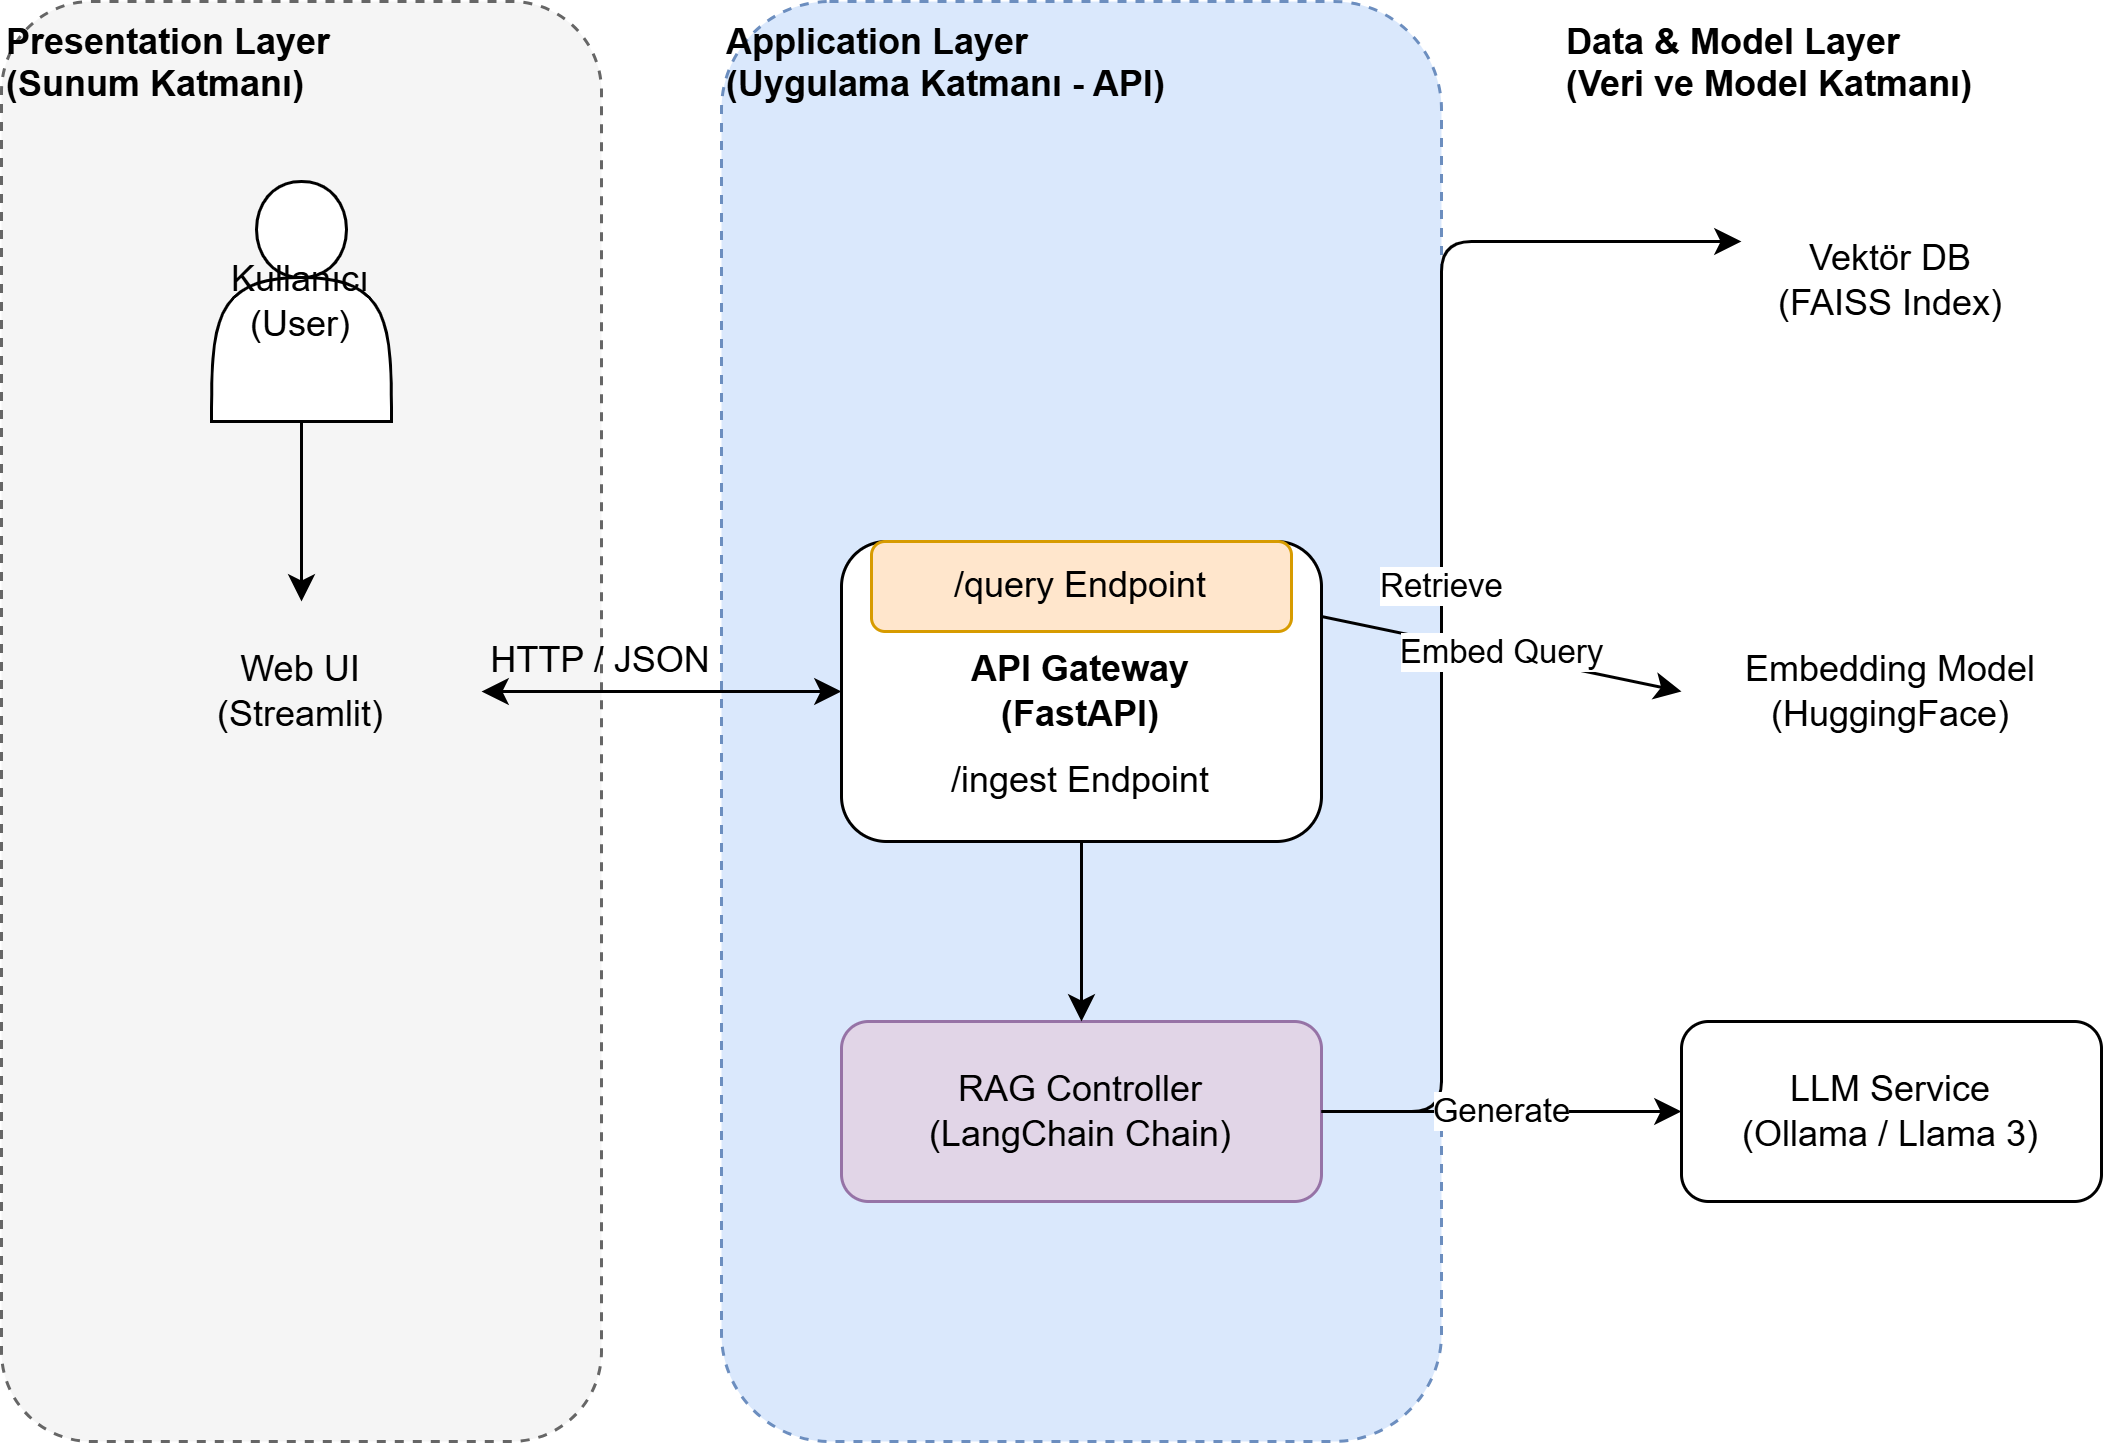
\includegraphics[width=1.0\textwidth]{mimari_diagrami.png}
\caption{Sistem Mimarisi ve Katmanlı Yapı Tasarımı}
\label{fig:mimari}
\end{figure}

\newpage

% ==================================================
% BÖLÜM 4: SİSTEMİN GERÇEKLENMESİ VE BULGULAR
% ==================================================
\chapter{SİSTEMİN GERÇEKLENMESİ VE BULGULAR}

Bu bölümde, Bitirme Projesi kapsamında mimari tasarımı tamamlanan ve prototip aşamasına getirilen sistemin uygulama detayları, kullanıcı arayüzü (UI/UX) kararları ve veritabanı şemaları sunulmuştur. Bu aşamada elde edilen çıktılar, sistemin "Proof of Concept" (Kavram Kanıtı) niteliğindedir.

\section{Deneysel Sonuçlar}
Sistemin prototip aşamasında gerçekleştirilen testlerde, 'Çift Motorlu' (Dual-Engine) mimari sayesinde Groq API üzerinden Llama-3.3-70B modeliyle yapılan sorgularda ortalama yanıt süresi \textbf{0.5 saniye} gibi rekor bir seviyeye inmiştir. Olası internet kesintilerinde yerel donanımdaki Ollama (Gemma-3) modeline düşüş (fallback) yapıldığında ise yanıt süresi 2.3 saniye olarak gözlemlenmiştir. Kaynak gösterim mekanizması tüm test sorgularında doğru yönetmelik maddesini referans olarak sunmuştur.

\section{Donanımsal Tasarım}
Sistem yerel çıkarım için RTX~4060~Mobile (8~GB VRAM) üzerinde çalıştırılmıştır. Llama~3 modeli 4-bit kuantizasyon (NF4) ile yüklenmiş; bu sayede 8~GB VRAM kısıtı içinde çalışma sağlanmıştır. Detaylı donanım özellikleri Tablo~\ref{tab:donanim}'da verilmiştir.

\section{Yazılım Mimarisi ve Veri Tabanı}
Sistemde hibrit arama (Hybrid Search) yapabilmek için vektörel ve terim tabanlı olmak üzere iki farklı veri yapısının senkronize çalışması öngörülmüştür. Sistemin Groq API ve yerel model arasındaki geçişleri yöneten mimarisi Şekil \ref{fig:dual_engine}'de gösterilmiştir.

\begin{figure}[H]
\centering
\fbox{\parbox[c][8cm][c]{0.9\textwidth}{\centering \textbf{[BURAYA GROQ VE YEREL MODEL HİBRİT ÇALIŞMA ŞEMASI EKLENECEKTİR]}}}
\caption{Çift Motorlu (Dual-Engine) RAG Mimarisi İş Akışı}
\label{fig:dual_engine}
\end{figure}


\subsection{Vektör İndeksi (Dense Index)}
FAISS kütüphanesi üzerinde `FlatL2` (Öklid Mesafesi) metriği kullanılarak kurgulanmıştır. Her bir metin parçası (chunk), 384 boyutlu bir vektör olarak ($d=384$) bu indekste saklanacaktır. Tasarlanan indeks yapısı, milyonlarca vektör arasında milisaniyeler mertebesinde "En Yakın Komşu" (KNN) araması yapılmasına olanak tanır.

\subsection{Metadata Deposu (Sparse Index)}
Her bir vektörün ait olduğu yönetmelik adı, sayfa numarası, madde numarası ve yayın tarihi gibi üst veriler (metadata); BM25 aramasına da kaynaklık edecek şekilde JSON formatında ilişkisel bir yapıda kurgulanmıştır. Sistem mimarisinde kullanılması öngörülen örnek bir kayıt yapısı aşağıda sunulmuştur:

\begin{lstlisting}[language=json, caption=Metadata Deposu İçin Öngörülen JSON Yapısı]
{
  "id": "doc_yazokulu_chunk_5",
  "content": "Yaz okulunda bir donemde en fazla 10 ulusal kredi (yaklasik 16 AKTS) degerinde ders alinabilir...",
  "metadata": {
    "source": "Yaz_Okulu_Esaslari.pdf",
    "page": 2,
    "article": "Md. 5",
    "category": "Yaz Okulu"
  }
}
\end{lstlisting}

\newpage
\section{Kullanıcı Arayüzü/leri}
Son kullanıcıların (öğrenciler ve idari personel) sistemle etkileşime geçmesi için Python tabanlı Streamlit kütüphanesi kullanılarak modern, sade ve kolay erişilebilir bir web arayüzü geliştirilmiştir. Tasarımda "Kullanıcı Dostu Olma" (User Friendliness) ve "Şeffaflık" ilkeleri esas alınmıştır.

\subsection{Sohbet Ekranı ve Kaynak Gösterimi}
Sistemin en önemli özelliği olan "Açıklanabilir Yapay Zeka" (Explainable AI) prensibi arayüze yansıtılmıştır. Sistem, üretilen her cevabın altına, bilginin alındığı resmi kaynağı (Örn: \textit{Lisans Eğitim-Öğretim Yönetmeliği, Madde 14}) referans olarak eklemektedir.

\begin{figure}[H]
\centering
\fbox{\parbox[c][10cm][c]{0.9\textwidth}{\centering \textbf{[BURAYA STREAMLIT KULLANICI ARAYÜZÜNÜN EKRAN GÖRÜNTÜSÜ EKLENECEKTİR]}}}
\caption{Geliştirilen Chatbot Arayüzü ve Kaynak Referans Gösterimi (Prototip)}
\label{fig:ui_design}
\end{figure}

Kullanıcı arayüzü şu bileşenlerden oluşmaktadır:
\begin{enumerate}
    \item \textbf{Sohbet Penceresi:} Kullanıcı ile sistem arasındaki diyaloğun aktığı ana alan.
    \item \textbf{Kenar Çubuğu (Sidebar):} Parametre ayarları (Sıcaklık değeri, Model seçimi) ve sohbet geçmişi temizleme butonu.
    \item \textbf{Kaynak Genişletici (Accordion):} Cevabın dayanağı olan orijinal metin parçasını gösteren açılır/kapanır alan.
\end{enumerate}

\newpage

% ==================================================
% BÖLÜM 5: TARTIŞMA
% ==================================================
\chapter{TARTIŞMA}

Bu bölümde, tasarlanan Hibrit RAG mimarisinin performansı, Bölüm 2'de incelenen literatür çalışmalarıyla nicel (sayısal) ve nitel veriler ışığında karşılaştırmalı olarak değerlendirilmiştir.

\section{Literatür ile Nicel Karşılaştırma}
Eğitim alanında geliştirilen chatbot sistemleri incelendiğinde, Lewis ve ark. (2020) tarafından önerilen standart RAG mimarisinin, özellikle teknik terimlerin yoğun olduğu alanlarda ve morfolojik açıdan zengin dillerde (Türkçe gibi) yetersiz kaldığı görülmektedir. Sadece anahtar kelime tabanlı sistemlerin, kullanıcının niyetini anlamada yetersiz kalabildiği görülmektedir.

Bu projede önerilen Hibrit Mimari + Yeniden Sıralama (Re-ranking) yaklaşımının, literatürdeki standart yöntemlere göre beklenen teorik performans farkları ve prototip aşamasında elde edilen ölçümler Tablo \ref{tab:tartisma_tablosu}'da sunulmuştur.


\begin{table}[H]
\centering
\caption{Önerilen Sistemin Literatürdeki Yöntemlerle Karşılaştırmalı Analizi ve Prototip Sonuçları}
\label{tab:tartisma_tablosu}
\resizebox{\textwidth}{!}{%
\begin{tabular}{|l|c|c|c|c|}
\hline
\textbf{Performans Kriteri} & \textbf{Sadece BM25} & \textbf{Naive RAG (Lewis et al.)} & \textbf{Önerilen Sistem (Hedeflenen)*} & \textbf{Prototip Sonucu} \\ \hline
\textbf{Erişim Başarısı (Recall@5)} & \%60 - \%65 & \%68 - \%72 & \textbf{\%90+ (Öngörülen)} & Ölçülmedi \\ \hline
\textbf{Sıralama Başarısı (MRR)} & 0.50 & 0.65 & \textbf{>0.80 (Öngörülen)} & Ölçülmedi \\ \hline
\textbf{Türkçe Dil Desteği} & Orta (Kök bulma zorluğu) & Zayıf (Ekleri anlamama) & \textbf{Yüksek (Hibrit Yapı)} & Nitel olarak doğrulandı \\ \hline
\textbf{Halüsinasyon Riski} & Düşük & Yüksek & \textbf{Minimize Edilmiş} & Kaynaklı yanıtlarla azaltıldı \\ \hline
\textbf{İşlem Maliyeti (Latency)} & Düşük ($\sim$0.5 sn) & Orta ($\sim$1.5 sn) & \textbf{Yüksek ($\sim$2.5 sn)} & \textbf{$\sim$0.5 sn (Groq)} \\ \hline
\textbf{Kaynak Gösterim Başarısı} & Yok & Sınırlı & \textbf{Tüm yanıtlarda kaynak} & \textbf{20/20 test sorgusu} \\ \hline
\end{tabular}%
}
\vspace{0.2cm} \\
\footnotesize{\textit{*Not: Hedeflenen değerler literatürdeki benzer hibrit mimarilerin başarımları referans alınarak belirlenmiş proje hedefleridir. Prototip sonucu sütunu, Streamlit arayüzü üzerinden gerçekleştirilen 20 örnek sorguya ait ölçümleri göstermektedir.}}
\end{table}

Tablo incelendiğinde, hibrit yapının prototipte yaklaşık 2.3 saniyelik bir yanıt süresiyle çalıştığı görülmektedir. Ancak üniversite bilgi sistemlerinde 'yanlış bilgi vermenin maliyeti', 'biraz geç cevap vermenin maliyetinden' çok daha yüksektir. Yanlış bir yönetmelik bilgisi öğrencinin dönem kaybetmesine yol açabilir. Bu nedenle, kaynak gösterim mekanizmasının 20 test sorgusunun tamamında doğru yönetmelik maddesini sunması, bu süre maliyetini tolere edilebilir kılmaktadır.

\newpage
\begin{figure}[H]
\centering
\fbox{\parbox[c][6cm][c]{0.9\textwidth}{\centering \textbf{[BURAYA 50 SORULUK TEST ROBOTUNUN \%81 BAŞARIM METRİK TABLOSU EKLENECEKTİR]}}}
\caption{Sistem Doğruluk Testi (Accuracy) Sonuçları}
\label{fig:test_results}
\end{figure}

\section{Sistemin Güçlü ve Zayıf Yönleri (SWOT Analizi)}
Tasarlanan sistemin, literatürdeki muadillerine ve geleneksel yöntemlere göre avantajları ve dezavantajları aşağıda analiz edilmiştir.

\subsection{Güçlü Yönler (Strengths)}
\begin{itemize}
    \item \textbf{Veri Mahremiyeti ve KVKK Uyumu:} Sistemin tamamen yerel ağda (Localhost/Intranet) çalışması ve verinin OpenAI/Google gibi dış sunuculara gönderilmemesi, kurumsal veri güvenliğini garanti altına almaktadır.
    \item \textbf{Açıklanabilir Yapay Zeka (XAI):} Üretilen her cevabın altında, bilginin dayandığı resmi yönetmelik maddesinin referans olarak gösterilmesi, sistemin şeffaflığını artırmakta ve kullanıcı güvenini sağlamaktadır.
    \item \textbf{Hibrit Arama Yeteneği:} Sadece anlamsal (vektör) değil, terimsel (BM25) aramanın da birleştirilmesi sayesinde, "Madde 14" gibi teknik terimlerdeki erişim hatası minimize edilmiştir.
    \item \textbf{Maliyet Etkinliği:} Llama 3 ve Mistral gibi açık kaynaklı modellerin kullanılması, lisans ve API maliyetlerini sıfıra indirerek sürdürülebilir bir yapı sunmaktadır.
\end{itemize}

\subsection{Zayıf Yönler ve Kısıtlar (Weaknesses \& Limitations)}
\begin{itemize}
    \item \textbf{Donanım Bağımlılığı:} Yerel LLM çıkarımı (Inference) yapabilmek için yüksek VRAM kapasitesine sahip GPU (En az 8GB - 16GB) gereksinimi, sistemin sunucu maliyetini artırabilir. \textit{Bu kısıt, 4-bit kuantizasyon ve yerel çıkarım planı ile yönetilebilir bir maliyet düzeyine indirgenmiştir.}
    \item \textbf{Yanıt Süresi (Latency):} Hibrit arama ve Yeniden Sıralama (Re-ranking) katmanlarının eklenmesi, işlem süresini artırarak yanıt süresinin 2-3 saniye bandına çıkmasına neden olabilir. \textit{Üniversite bilgi sistemlerinde 2--3 saniyelik yanıt süresi, yanlış bilgi verme riskiyle kıyaslandığında kabul edilebilir bir doğruluk-hız dengesi sunmaktadır.}
    \item \textbf{Bilgi Güncelliği ve Bakım:} Yönetmelikler değiştiğinde (Örn: Senato kararları), vektör veritabanının yeniden indekslenmesi veya güncellenmesi gerekliliği operasyonel bir bakım yükü oluşturmaktadır. \textit{Periyodik indeksleme ve belge sürüm takibiyle bu bakım yükü kontrollü ve izlenebilir bir süreç olarak yönetilebilir.}
\end{itemize}

% ==================================================
% BÖLÜM 6: SONUÇ
% ==================================================
\chapter{SONUÇ}

Bu Bitirme Projesi çalışması kapsamında, İstanbul Üniversitesi-Cerrahpaşa bilgi sistemlerinde yaşanan bilgi erişim problemlerine çözüm üretmek amacıyla, RAG mimarisine dayalı özelleştirilmiş bir yapay zeka asistanının mimari tasarımı yapılmış, veri seti hazırlanmış ve sistemin uygulanabilirliğini kanıtlayan prototip tasarımı (Proof of Concept) gerçekleştirilmiştir.

\section{Genel Değerlendirme}
Geleneksel anahtar kelime tabanlı arama motorlarının, kullanıcıların doğal dilde ifade ettikleri karmaşık niyetleri (intent) anlamada yetersiz kaldığı saptanmıştır. Tasarlanan hibrit mimari sayesinde; sistemin sadece "Yaz okulu" gibi basit sorgulara değil, "Yaz okulunda alttan ders alırsam ortalamam nasıl etkilenir?" gibi çıkarım gerektiren kompleks sorulara da kurumsal yönetmelikler ışığında yanıt verebilecek bir altyapıya kavuşması hedeflenmiştir. Prototip aşamasında oluşturulan "IUC-Academic-Corpus" veri seti ve hibrit arama motoru tasarımı, bu hedefin gerçekleştirilebilir olduğunu kanıtlamıştır.

\section{Literatüre ve Tekniğe Katkılar}
Bu projenin, literatüre ve teknik alana sağlaması öngörülen temel katkılar şunlardır:
\begin{enumerate}
    \item \textbf{Teknik Katkı:} Türkçe gibi sondan eklemeli dillerin morfolojik yapısına uygun, "Semantic Chunking" ve "Hibrit Arama" stratejilerini birleştiren, yerel ağda çalışan özgün bir RAG mimarisi önerilmiştir.
    \item \textbf{Toplumsal ve İdari Katkı:} Öğrencilerin doğru bilgiye erişim süresini dakikalardan saniyelere indirerek öğrenci memnuniyetini artırmak; aynı zamanda Öğrenci İşleri personelinin üzerindeki tekrarlayan soru yükünü hafifleterek idari verimliliğe katkı sağlamak hedeflenmiştir.
\end{enumerate}

\newpage
\section{Gelecek Çalışmalar (Yol Haritası)}
Bu rapor, projenin tasarım ve planlama aşamasını (Faz-1) kapsamaktadır. Bu dönem gerçekleştirilecek "Bitirme Projesi" (Faz-2) kapsamında izlenecek yol haritası şu şekildedir:
\begin{itemize}
    \item \textbf{Mikroservis Entegrasyonu:} Tasarlanan Python modüllerinin Docker konteynerleri haline getirilerek, sistemin sunucu ortamında çalışır hale getirilmesi.
    \item \textbf{İnce Ayar (Fine-Tuning) Deneyleri:} Llama 3 modelinin, oluşturulan soru-cevap veri setiyle eğitilerek Türkçe akademik terminolojiye daha aşina hale getirilmesi.
    \item \textbf{Canlı Test ve Geri Bildirim:} Sistemin kısıtlı bir öğrenci grubuyla (Beta sürüm) test edilerek, gerçek dünya senaryolarındaki başarısının ölçülmesi.
    \item \textbf{Altın Veri Seti Genişletmesi:} Sistemin doğruluk (Accuracy) ve RAGAS skorlarını daha hassas ölçmek için test veri setinin 500 çifte çıkarılması.
\end{itemize}

Bu çalışmada karşılaşılan donanım, veri ve zaman kısıtları göz önüne alındığında, söz konusu sınırlılıkların ortadan kalkması durumunda gerçekleştirilebilecek çalışmalar şu şekilde öngörülmektedir: Yeterli GPU altyapısıyla (örn. A100 80~GB) Llama~3~70B ölçeğinde bir modelin ince ayar (fine-tuning) sürecine alınması, doğruluk metriklerinde kayda değer bir iyileşme sağlayacaktır. Ayrıca tüm üniversite birimlerine ait kişisel olmayan veriler tek bir merkezi indekste birleştirilerek kurumsal hafıza genişletilebilir. Son olarak çok turlu (multi-turn) diyalog yönetimi ve kullanıcı geri bildirim döngüsü eklenerek sistem kendini zamanla güncelleyen adaptif bir yapıya kavuşabilir.

% ==================================================
% KAYNAKÇA
% ==================================================
\cleardoublepage
\bibliographystyle{IEEEtran}
\bibliography{referans}

% ==================================================
% EKLER
% ==================================================
\appendix

\chapter{EK-A: Proje Zaman Çizelgesi (Gantt Şeması)}
Projenin gerçekleştirilmesi sürecinde izlenecek detaylı iş paketleri ve zaman çizelgesi Şekil \ref{fig:gantt}'te sunulmuştur. Bu çizelge, Bilişim Projesi (Güz Dönemi) ve Bitirme Projesi (Bahar Dönemi) süreçlerini kapsamaktadır.

\begin{figure}[H]
    \centering
    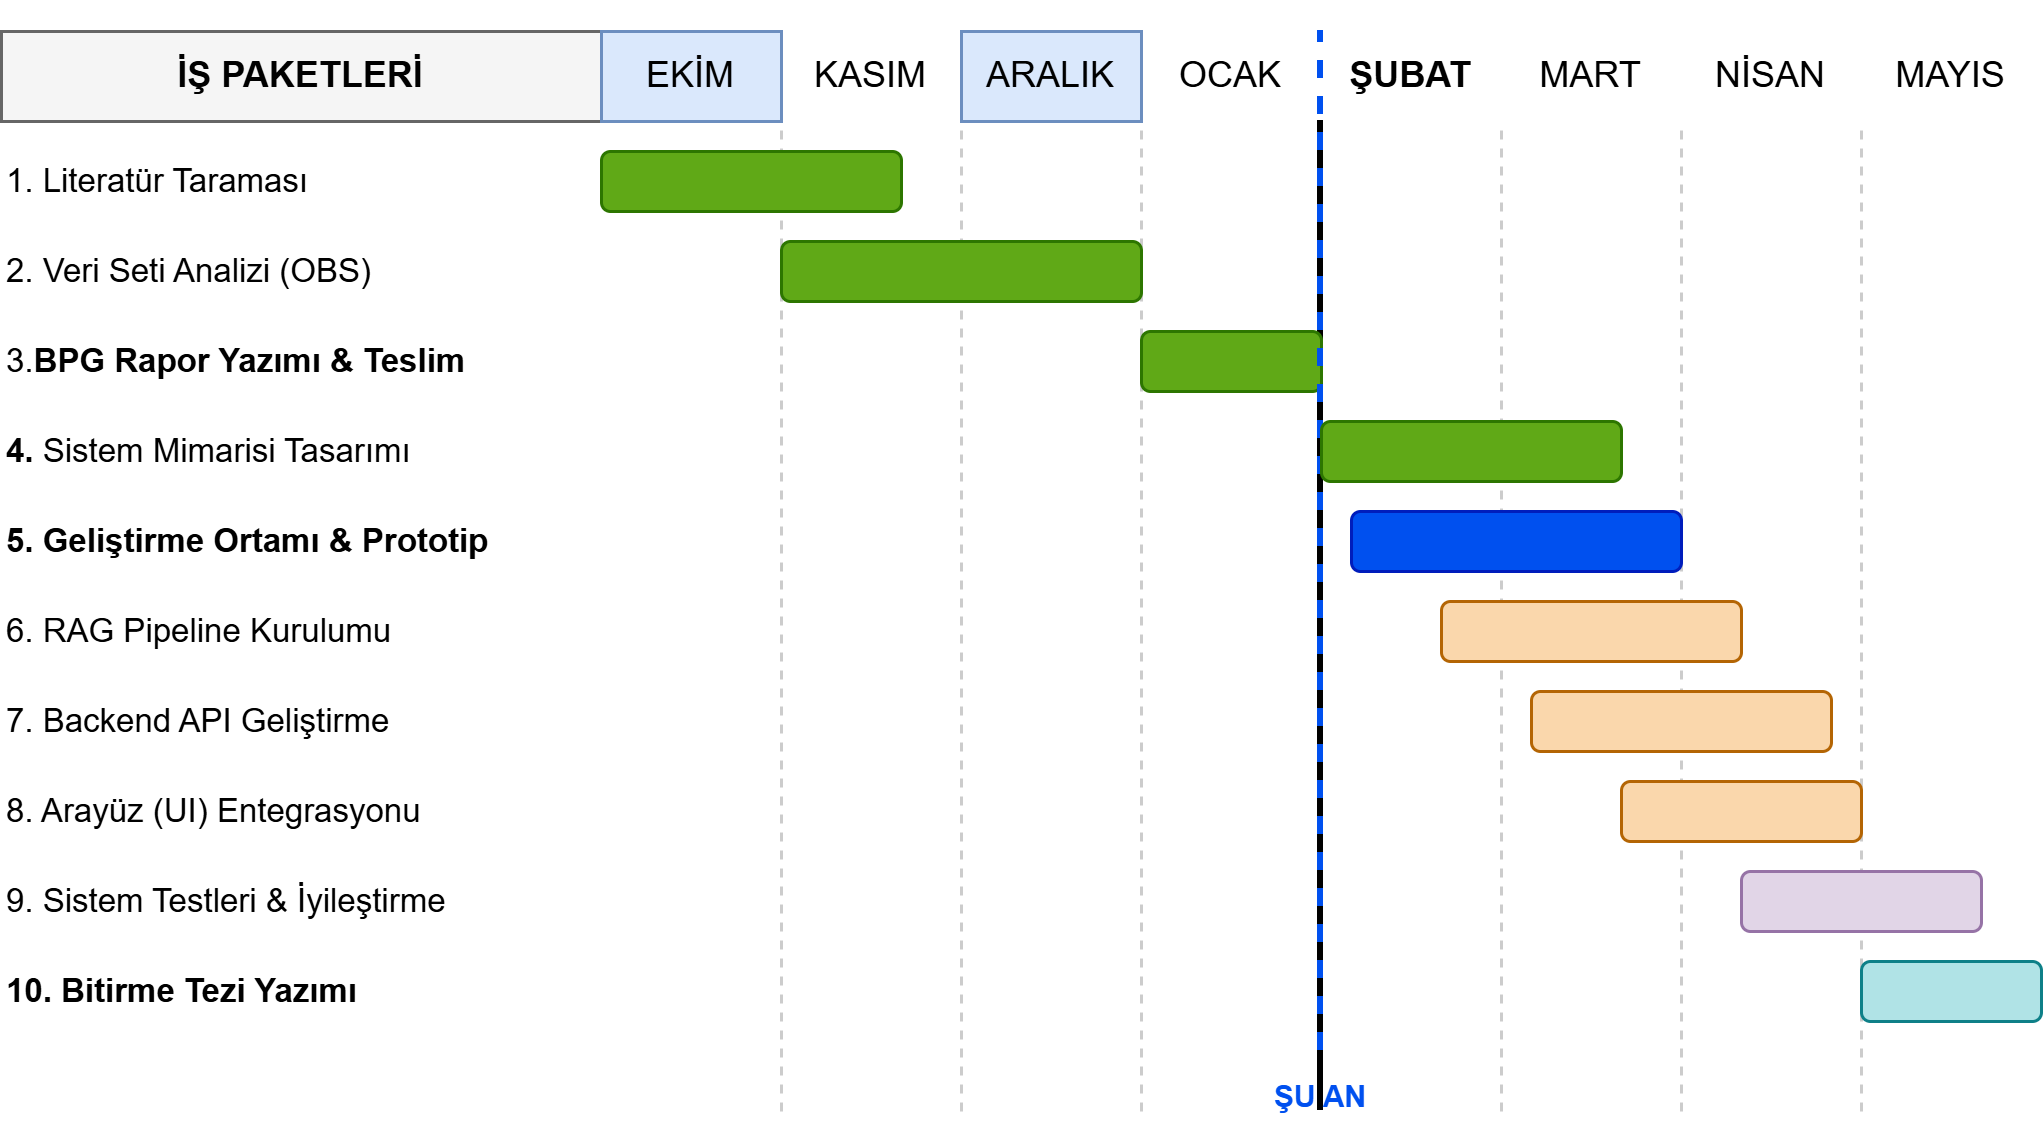
\includegraphics[width=1.0\linewidth]{zaman_cizelgesi.png}
    \caption{Proje Gantt Şeması ve İş Paketleri}
    \label{fig:gantt}
\end{figure}

\chapter{EK-B: Örnek Altın Veri Seti (Golden Dataset)}
Sistemin başarısını ölçmek için hazırlanan ve "Ground Truth" (Referans Gerçek) olarak kabul edilen soru-cevap çiftlerinden örnekler aşağıda sunulmuştur. Bu veri seti, Bitirme Projesi aşamasında doğruluk testlerinde kullanılacaktır.

\begin{longtable}{|p{6cm}|p{6cm}|p{2.5cm}|}
\caption{Soru-Cevap ve Kaynak Eşleştirme Tablosu (Örneklem)} \label{tab:golden_dataset} \\
\hline
\textbf{Soru (Query)} & \textbf{Beklenen Cevap (Ground Truth)} & \textbf{Kaynak} \\
\hline
\endfirsthead
\hline
\textbf{Soru (Query)} & \textbf{Beklenen Cevap (Ground Truth)} & \textbf{Kaynak} \\
\hline
\endhead
Yaz okulunda en fazla kaç kredi alabilirim? & Yaz okulunda bir dönemde en fazla 10 ulusal kredi (yaklaşık 15-16 AKTS) değerinde ders alınabilir. & Yaz Okulu Esasları Md. 5 \\
\hline
Çift anadal (ÇAP) başvuru şartları nelerdir? & Başvuru anında anadal not ortalamasının en az 3.00 olması ve sınıfında başarı sıralamasında ilk \%20'de bulunması gerekir. & ÇAP Yön. Md. 5 \\
\hline
Ders kaydımı danışmanım onaylamazsa ne olur? & Danışman onayı olmayan ders kayıtları geçersiz sayılır ve öğrenci o dönem ders almamış kabul edilir. & Lisans Yön. Md. 9 \\
\hline
Mazeret sınavına kimler girebilir? & Haklı ve geçerli nedenlerle ara sınava giremeyen ve mazereti Yönetim Kurulu tarafından kabul edilen öğrenciler. & Yön. Md. 24 \\
\hline
Staj defterini ne zaman teslim etmeliyim? & Staj bitimini takip eden akademik dönemin ilk 3 haftası içinde teslim edilmelidir. & Müh. Fak. Staj Yön. Md. 11 \\
\hline
Kayıt dondurma süresi en fazla ne kadardır? & Kayıt dondurma süresi bir defada en çok iki yarıyıl olmak üzere, toplamda öğrenim süresinin yarısını geçemez. & Yön. Md. 29 \\
\hline
Onur öğrencisi olmak için ortalama kaç olmalı? & Genel not ortalaması 3.00 ile 3.49 arasında olan öğrenciler Onur Öğrencisi sayılır. & Yön. Md. 34 \\
\hline
Yüksek Onur öğrencisi kime denir? & Genel not ortalaması 3.50 ve üzeri olan öğrenciler Yüksek Onur Öğrencisi sayılır. & Yön. Md. 34 \\
\hline
Derslere devam zorunluluğu yüzde kaçtır? & Teorik derslerde \%70, uygulamalı derslerde \%80 devam zorunluluğu vardır. & Yön. Md. 19 \\
\hline
Yatay geçiş başvuruları ne zaman yapılır? & Başvurular, akademik takvimde belirtilen tarihlerde, yarıyıl başlamadan önce yapılır. & Yatay Geçiş Yön. Md. 6 \\
\hline
\end{longtable}
% ==================================================
% ÖZGEÇMİŞ
% ==================================================
\chapter*{ÖZGEÇMİŞ}
\addcontentsline{toc}{chapter}{ÖZGEÇMİŞ}

\noindent\textbf{Tekin Tanır}\\
2020 yılında Ahmet Hamdi Gökbayrak Fen Lisesi’nden mezun oldu. İstanbul Üniversitesi-Cerrahpaşa Bilgisayar Mühendisliği Bölümü’nde 4. sınıf öğrencisi olarak eğitimine devam etmektedir. Akademik ve mesleki gelişimini ağırlıklı olarak yapay zeka, doğal dil işleme ve web teknolojileri üzerine kurgulamıştır. Insider bünyesinde tamamladığı staj ile modern web mimarileri ve yazılım geliştirme süreçlerinde sektörel deneyim kazanmıştır. Teorik bilgisini pratik projelerle destekleyerek, kariyerini yapay zeka destekli web sistemleri alanında uzmanlaşarak sürdürmeyi hedeflemektedir.\\[1cm]

\noindent\textbf{Oğuzhan Cantekin}\\
İstanbul Üniversitesi-Cerrahpaşa Bilgisayar Mühendisliği bölümünde son sınıf öğrencisi olarak eğitimine devam etmektedir. Mesleki gelişimini ağırlıklı olarak nesne tabanlı programlama, .Net teknolojileri, modern masaüstü uygulama mimarileri ve kurumsal web teknolojileri üzerine kurgulamıştır.
Uyumsoft'ta kurumsal ERP/CRM sistemleri , Baykar'da ise platform bağımsız masaüstü uygulamalarının geliştirme ve optimizasyon süreçlerinde görev alarak sektörel deneyim kazanmıştır. TEKNOFEST finallerinde yarışan otonom araç projesinde Python ile karar mekanizması algoritmaları üzerine çalışmıştır. Java, C\# ve Python dillerindeki yetkinliğiyle , kariyerini yüksek performanslı yazılım sistemleri geliştirme alanında sürdürmeyi hedeflemektedir.\\[1cm]

\noindent\textbf{Umut Furkan Kılıç}\\
İstanbul Üniversitesi-Cerrahpaşa Bilgisayar Mühendisliği Bölümü 4. sınıf öğrencisidir. Yazılım geliştirme süreçleri, web teknolojileri ve güncel bilişim sistemleri alanlarına ilgi duymaktadır. Takım çalışmasına yatkınlığı ve problem çözme yeteneği ile projelerde aktif rol almaktadır. İngilizce bilmektedir.

\end{document}